\documentclass[12pt,letterpaper]{article}
\usepackage{anysize}
%\usepackage[spanish, es-tabla]{babel}
%\usepackage[spanish]{babel}
\usepackage[utf8]{inputenc}
\renewcommand{\familydefault}{\sfdefault}
\usepackage{graphicx}
\usepackage{color}
\usepackage{amssymb}
\usepackage{url}
\usepackage{float}
\usepackage{fancyhdr}
\usepackage{nccmath}
\usepackage{hyperref}
\usepackage{epstopdf}
\usepackage{subfig}
\usepackage{anysize} 
\usepackage{wrapfig}
\usepackage{listings}
\usepackage{setspace}
\usepackage{multicol}
\usepackage{tabularx}
\usepackage[titletoc,toc,page]{appendix}
\numberwithin{figure}{section}
\numberwithin{equation}{section}
\numberwithin{table}{section}
% \spanishdecimal{,}
\marginsize{3cm}{3cm}{1cm}{1cm}
\setcounter{totalnumber}{3}
\newcommand{\HRule}{\rule{\linewidth}{0.5mm}}
\usepackage{hyperref}
\newcolumntype{L}[1]{>{\raggedright\arraybackslash}p{#1}}
\newcolumntype{C}[1]{>{\centering\arraybackslash}p{#1}}
\newcolumntype{R}[1]{>{\raggedleft\arraybackslash}p{#1}}
\usepackage[normalem]{ulem}
\useunder{\uline}{\ul}{}


%\apptocmd{\bibliography}{\csname phantomsection\endcsname\addcontentsline{toc}{chapter}{\bibname}}{}{}

\usepackage[table,xcdraw]{xcolor}
\usepackage[section]{placeins}
\makeatletter
\AtBeginDocument{%
  \expandafter\renewcommand\expandafter\subsection\expandafter{%
    \expandafter\@fb@secFB\subsection
  }%
}
\makeatother
\makeatletter
\AtBeginDocument{%
  \expandafter\renewcommand\expandafter\subsubsection\expandafter{%
    \expandafter\@fb@secFB\subsubsection
  }%
}
\makeatother


\begin{document}
\newpage

\pagestyle{fancy}
\fancyhf{}
\renewcommand{\headrulewidth}{0pt}
\fancyhead[R]{ 
\includegraphics[scale=0.2]{logo_escudo_eps.eps} }
%\fancyhead[L]{ \includegraphics[scale=0.2]{dimec_eps.eps} }

\vspace*{6cm}
\begin{center}
% AOT retrieval procedure for distributed measurements with low cost Sun Photometers

{


\huge Open Source LED Sun Photometer Construction and Operation Manual\\
\vspace{0.5cm}

}

%\vspace{1.5cm}
%{\large CONSTRUCTION MANUAL\\
%ME5601-1 \\ }

\vspace{11cm}

{
{
Supplementary material for the document "AOT retrieval procedure for distributed measurements with low cost Sun Photometers"\\ December 2016, University of Chile, Santiago, Chile.
}
}
\end{center}


\newpage
\marginsize{3cm}{3cm}{-1cm}{2cm} 
\pagestyle{fancy}
\fancyhf{}

\fancyhead[L]{ \rm \textit{Content}} 

\renewcommand{\sectionmark}[1]{\markright{\thesection.\ #1}}
\renewcommand{\headrulewidth}{0.5pt}


\onehalfspace
\tableofcontents



\newpage
\fancyhead[L]{ \rm \textit{Section \rightmark}}
%\fancyhead[L]{ }
\setcounter{page}{1}
\renewcommand{\headrulewidth}{0.5pt}
\fancyfoot[R]{\small \rm \textit{\thepage  }}
\renewcommand{\footrulewidth}{0.pt}

%\section{Introducci├│n}

%\subsection{Antecedentes}

%\subsection{Motivaci├│n}

%\newpage
\section{Introduction}



\subsection{Aerosols}

Aerosols are molecules or particles (solids and/or liquids) suspended on the atmosphere, that disperse and absorb sunlight, affecting the intensity of radiation that is perceived on Earth's surface. The effect of the dispersion and absorption on direct radiation from the Sun can be theoretically calculated as function of wavelength. The reduction in direct radiation is described through the optical thickness, the greater the dispersion and absorption, the greater the value of the optical thickness \cite{Brooks}. The contribution of dispersion and absorption to the reduction of direct radiation is linearly proportional to (1) the intensity of radiation measured along the path traveled by the light, (2) the local concentration of the aerosol, and (3) the efficiency of dispersion and absorption \cite{wallace2008}.

The basic equation governing the transmission of radiation through a medium is known as the Law of Beer (Eq. (\ref{eq:1})).

\begin{equation}
    I_\lambda=I_{o,\lambda}\exp(-\alpha_\lambda m_{air})
    \label{eq:1}
\end{equation}

where $I_{o,\lambda}$ is the source original light intensity, $I_\lambda$, is the light intensity after passing through the relative air mass $m_{air}$, and $\alpha_\lambda$ is the total atmospheric optical thickness factor (including molecular dispersion, and dispersion and absorption due to gases and aerosols), at the wavelength $\lambda$. The relative air mass defines the length of the direct optical path through the atmosphere, expressed as the ratio relative to the length of the vertical path (in zenith); The value of the relative air mass is shown in the Eq. (\ref {eq:2})

\begin{equation}
    m_{air}=\frac{L}{L_0}\approx\frac{1}{\cos(z)}
    \label{eq:2}
\end{equation}


where $L$ is the length of the path through the atmosphere, $L_0$ is the zenith length of the path (normal to the Earth's surface) and $z$ is the zenithal angle.

The total optical thickness is composed of molecular dispersion (Rayleigh), the absorption of gases (ozone and water vapor), and the dispersion and absorption due to aerosols (Eq. (\ref{eq:3}).

\begin{equation}
    \alpha_\lambda = \alpha_{\lambda,R} + \alpha_{\lambda,g} + \alpha_{\lambda,a}
    \label{eq:3}
\end{equation}

where Eq. (\ref{eq:3}) is written for a specific wavelength $\lambda$. The value of $\alpha_{\lambda,R}$ (Rayleigh) can be calculated using atmospheric models. One way of calculating the value of $\alpha_{\lambda,R}$ is proposed by \cite{Bucholtz}:

\begin{equation}
    \alpha_{\lambda,R} = \frac{P}{P_0}A\lambda^{(-B-C\lambda-D/\lambda)}
    \label{eq:4}
\end{equation}

where $(P/P_0)$ is the ratio between the measured pressure at the site and the standard atmospheric pressure at sea level, and $\lambda$ is the wavelength in micro meters. The parameters $A$, $B$, $C$, and $D$ are equation coefficients with values shown in the Table \ref{tab:1}, which give the best fit to theoretical calculations.

\begin{table}[H]
\centering
\caption{ Coefficients for the Rayleigh optical thickness calculation \cite{Bucholtz}.}
\label{tab:1}
\begin{tabular}{|l|r|r|}
\hline
Coeficiente & \multicolumn{1}{l|}{$\lambda\leq0.500$ $\mu m$ ($500$ $nm$)} & \multicolumn{1}{l|}{$\lambda>0.500$ $\mu m$ ($500$ $nm$)} \\ \hline
A & $6.50362\times10^{-3}$ & $8.64627\times10^{-3}$  \\ \hline
B & $3.55212$              & $3.99668$               \\ \hline
C & $1.35579$              & $1.10298\times10^{-2}$  \\ \hline
D & $0.11563$              & $2.71393\times10^{-2}$  \\ \hline
\end{tabular}
\end{table}

\subsection{Light Emitting Diodes (LEDs) as photo diodes}

A device that operates as a light sensor is known as a photodiode, which is defined as a transducer from optical to electrical energy producing a current proportional to the received light. On the other hand, LEDs emit light by applying a current flow through it. Since the imposed charge carries electrons and holes, when an electron encounters a hole it falls to a lower energy level releasing energy as a photon.

By placing a LED in inverted polarization, the inverse process occurs. So that when a LED in inverse polarization receives light it can absorb a photon, which is converted to an electron-hole pair. This generated electron-hole pair is free to move through the semiconductor under an electric field, producing an output current. Therefore, a LED can be also used as a photodiode.

\subsection{Estimation of Aerosol Optical Thickness (AOT)}

To estimate AOT using a LED as a light detector, the \textit{equivalent wavelength approximation} described in \cite{BrooksMims} is used, which can be summarized in the Eq. \ref{eq:001},

\begin{equation}
    \alpha_a = \frac{\ln\left(V_0\left(\frac{R_0}{R}\right)^2\right) - \ln\left( V \right) - \alpha_R \frac{P}{P_0} \cdot m_{air} }{ m_{air} } - \alpha_g
    \label{eq:001}
\end{equation}

where $\lambda$ is the monochrome wavelength of the light ray, $V$ is the measured voltage at the terminals of the LED (operating as a photodiode), $V_0$ is a calibration constant (it represents an estimate of the sensor response in case of no atmosphere), $(R_0/R)^2$ is the correction for the distance Earth-Sun (this term compensates for the effect of the variation of the radiation power received due to the distance variation to the Sun), $m_{air}$ is the relative air mass (represents the length of the path of light covered going through the atmosphere relative to a vertical path), $P$ is the pressure value measured at the measurement site, $P_0$ is the pressure at the see level, $\alpha_g $ is the optical thickness due to gases (GOT), $\alpha_R$ is the optical thickness of Rayleigh (ROT), $\alpha_a$ is the optical thickness of aerosols (AOT). The effect of the gases on the LEDs is not negligible (due to the broad spectral response of the LEDs). In particular, the yellow LED is affected by water vapor and ozone, although the effect is more relevant form the later.


\newpage
\section{Prototype description}

\subsection{General description}

The prototype photometer is composed of two LED sensors, used as photodiodes to measure the Sun's light, a computing system based on an Arduino platform, and a mechanical structure. LEDs receive light from the Sun, producing at their terminals an analog voltage, which is digitized using an analog pin and the internal Analog/Digital Converter (ADC) of the Arduino platform. The Arduino platform is connected to a Data Logger Shield that records the digitized voltage samples on a micro SD memory card.

The main parts of the photometer prototype are shown in Figure \ref{fig:1} (exterior view) and in Figure \ref{fig:2} (interior view). Table \ref{tab:2} summarizes the main components of the prototype divided into structural components and electrical components. Annex \ref{anexo:1} shows a detail of the materials and components necessary for the construction of the prototype. An online repository containing all the code and printable pieces has been enabled, in the website \url{https://github.com/FelipeToledo/DIY-SunPhotometer-UChile}.

The external structure is divided as follows:

\begin{enumerate}
    \item Control panel (Figure \ref{fig:1}(a)): interface that allows interaction with the prototype. Through the buttons the functions are activated and the voltage values of the measurements are displayed on the screen.
     \item Sun pointing system (figure \ref{fig:1}(b)): tabs on the side of the control panel perforated in the center. These holes are used to find the correct orientation of the instrument with respect to the Sun to properly measure AOT.
     \item Switch (Figure \ref{fig:1}(c)): prototype on/off button.
     \item Light entrance (Figure \ref{fig:1}(d)): perforations at one end of the prototype that allow the light to enter to the instrument and reach the LED sensors.
     \item Tripod adapter (Figure \ref{fig:2}(a)): allows to install the prototype on a tripod as support.
\end{enumerate}

The internal parts of the prototype can be divided as follow:

\begin{enumerate}
     \item Battery (Figure \ref{fig:2}(b)): it provides energy to the prototype.
     \item Arduino (Figure \ref{fig:2}(c)): it is micro-processing platform. We use a construction kit sold by MCI Electronics in Chile called Armaduino. The main function of this sub-system is to sample the voltage at the LEDs terminals and digitize those samples.   
     \item Data logger (Figure \ref{fig:2}(c)): It is used to record the digitized voltages samples as they progress with time. Date, time and digitized voltages are saved in a micro SD memory stick.
     \item Sensor (Figure \ref{fig:2}(d)): LEDs used as photodiodes.
\end{enumerate}

\begin{figure}[!htb]
    \centering
    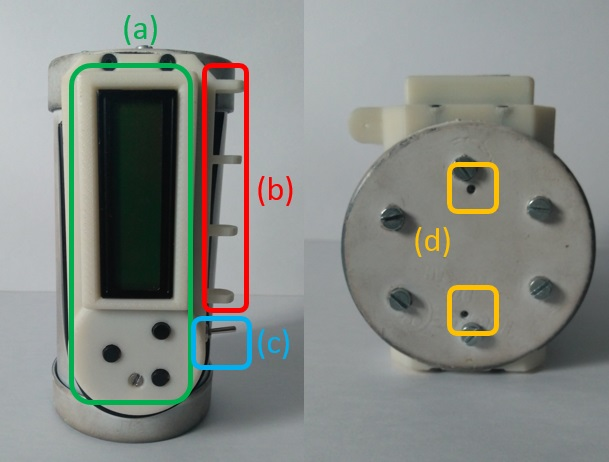
\includegraphics[scale=0.75]{Figuras/figure_1.jpg}
    \caption{External view of the Sun photometer: (a) Control Panel, (b) Sun pointing system, (c) Switch on/off, (d) Light entrance.}
    \label{fig:1}
\end{figure}

\begin{figure}[!htb]
    \centering
    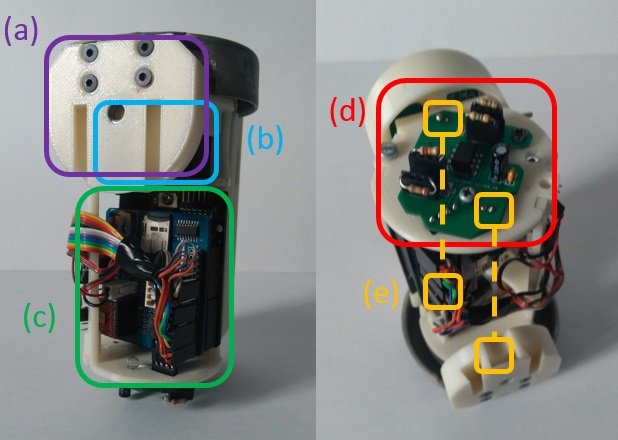
\includegraphics[scale=0.75]{Figuras/figure_2.jpg}
    \caption{Left Image: (a) Tripod adapter, (b) Battery, and (c) Arduino with Data Logger. Right Image: (d) LED Sensors board, (e) Location of the LED sensors (top yellow squares in the image) and light entrance holes (bottom yellow squares in the image).}
    \label{fig:2}
\end{figure}

\begin{table}[!htb]
\centering
\caption{Components and materials used by the Sun photometer prototype.}
\label{tab:2}
\begin{tabular}{|l|l|}
\hline
\textbf{Structural Components}    & \textbf{Material} \\ \hline
Control Panel (structure)         & ABS               \\ \hline
Sun pointing system               & ABS               \\ \hline
Tripod adapter                    & ABS               \\ \hline
External case                     & PVC               \\ \hline
Internal structure                & ABS               \\ \hline
\textbf{Electronic Components}    & \textbf{}         \\ \hline
PCB Interface                     &                   \\ \hline
LCD screen                        &                   \\ \hline
Sensor PCB board                  &                   \\ \hline
Arduino                           &                   \\ \hline
Data Logger shield with micro SD card &                   \\ \hline
DS1307 Real Time Clock Shield     &                   \\ \hline
Pressure and temperature sensor BMP180 &                   \\ \hline
LEDs                              &                   \\ \hline
9V Battery                        &                   \\ \hline
\end{tabular}
\end{table}



%%%%%% DESCRIBIR PROTOTIPO FOTOMETRO %%%%%%

\subsection{Operation Procedure}

The operation of the prototype starts by turning the instrument on with the switch. If the system is operating correctly, a message on the screen will be displayed and keeping awaiting for the user's actions. The buttons on the control panel allow you to perform three actions: (1) \textit{Test mode} (upper left button), (2) \textit{Measuring mode} (bottom button), (3) \textit{Data extraction mode} (upper right button).

The \textit{Test mode} allows practicing the use of the prototype to find the optimal orientation to measure AOT. On the screen the maximum voltage value obtained in each sensor is updated. The \textit{Measurement mode} performs a process that lasts 14 seconds and registers 400 voltage data per second. The maximum value, during these 14 seconds, at each sensor are stored in the Data logger. These maximum values (one per each LED) are the one shown on the screen at the end of the process. Thus, the sun photometer has not to be fixed pointing towards the Sun, but the user has to move it during this 14 seconds period trying to be sure in some moment the photometer was properly pointed. The \text{Data extraction mode} allows to obtain the measurements stored on the micro SD card of the Data logger in a .csv file. Once the action done with one of the buttons is finished, just press another button to perform the next action.

To perform a measurement it is recommended to follow the following steps:

\begin{itemize}
	\item Turn on the Sun photometer.
	\item Point to the Sun, with the edge of the prototype where the light inputs (or holes) are.
	\item Move the Sun photometer so that the ray of light passes through all and each of the tabs' holes. Thus, the Sun beam should be seen in the center of the last tab.
	\item Press the \textit{Measure mode} button to start the measurement. \textbf{t is recommended to slightly move the instrument so that the light spot over the last tab moves around the tab center. It is done to be sure the light beam reaches the LEDs. For a human it is hard to keep still pointing to the Sun without any natural oscillation. In addition, this movement can compensate for slightly deviations between the pointing system (the tabs) and where the actual light is hitting inside the instrument.}
	\item \textbf{Repeat the procedure according to the desired number of measurements to be performed. It is advisable to perform more than one measurement in a time range of 2 minutes to ensure that the maximum value is actually measured on both sensors).}
\end{itemize}

After each measurement process it is recommended to switch off the instrument to extend the life of the battery. In addition, while possible, leave the instrument covered and in the shade to avoid the wear of any of the components.



%*************************************************************INICIO FELIPE**************************************************

\subsection{Systems}

% Mi translation (FELIPE TOLEDO)
\subsubsection{Electronic components}
 \label{componentes_electronicos}
 
\begin{flushleft}
\textbf{(i) Aerosol Sensor}
\end{flushleft}

The objective of the sensor is to quantify the light intensity received from the sun in a small wavelength span which is determined by the LEDs used. LEDs generate a current linearly proportional to the light intensity they receive in their wavelenght sensitivity band.

In most cases the current generated by the LED is small, in the order of the microamperes. Because of this the use of an amplifier circuit is escential. The function of this circuit is to map this small current into a larger voltage signal, which must be within a range easy to measure and register.

The amplifier circuit is composed by a TLC272 Operational Amplifier, which is powered using the 5 [V] source from the Armaduino board. The output of the circuit is an analog voltage within the range of 0 to 4.2 [V]. This signal is transmited to the pin A1 of the Armaduino board. Pin A1 has an analog to digital converter (ADC) capable to measure voltages in the range between 0 and 5 [V] with a 10 bit resolution.

Figure \ref{fig:3} shows the sensor circuit components. The resistances shown in Figure \ref{fig:3} are of a referential value and depend on the model of LED used. These resistances allow the modification of the amplification magnitude following the next relationship:

\begin{equation}
    V_{measured} = 2R_1I_{LED}
    \label{eq:5}
\end{equation}

Considering the fact that the amplifier output range is limited it is important to limit the value of $R_1$ so that the sensor doesn't reach the saturation level in the output (4.2 [V]) under operative conditions. The inclusion of two resistance sockets in series for the amplification feedback allows a more flexible determination of the resistance values to use in the circuit. 


\begin{figure}[H]
    \centering
    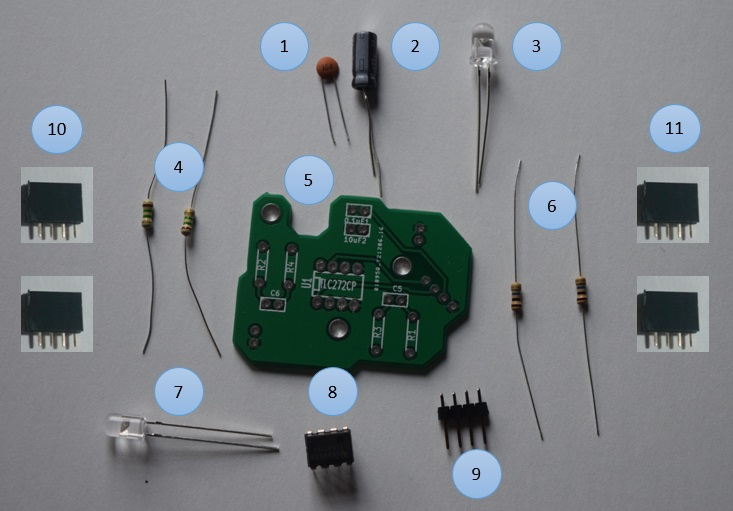
\includegraphics[scale=0.75]{Figuras/figure_3.jpg}
    \caption{Aerosol sensor components: (1) Capacitor 0.1 [$\mu$F], (2) Capacitor 10 [$\mu$F], (3) Yellow LED, (4) Resistance 1.5 [M$\Omega$], (5) Sensor PCB, (6) Resistance 10 [M$\Omega$], (7) Blue LED, (8) TCL272CP, (9) Male Pin Header 4x1, (10,11) Female Pin Header 4x1.}
    \label{fig:3}
\end{figure}

Female pin headers are soldered to the sensor PCB in the R1, R2, R3 and R4 footprints. This way it will be possible to interchange resistances easily by connecting and disconnecting them from the pin connector. This is usefull to test different amplification configurations. Figure \ref{fig:4} shows how to properly connect the resistance. It is important to note that before soldering this connector to the PCB the two middle copper connectors must be removed.

\begin{figure}[H]
    \centering
    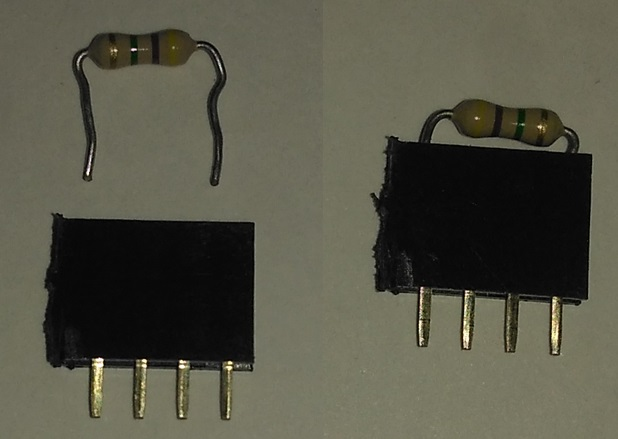
\includegraphics[scale=0.5]{Figuras/figure_4.jpg}
    \caption{Resistance connection on the female pin header 4x1.}
    \label{fig:4}
\end{figure}

To determine the best resistances configuration it is recommended to follow the next procedure: Measure the maximum output voltage of the sensor at noon (solar maximum height in the sky) with a clear line of sight to the sun. $R_1$ of equation \ref{eq:5} must be tuned to obtain an output signal of $\approx 75\%$ of the maximum output in the aformentioned conditions.

In the following pages the location of the sensor PCB components is explained, using the board footprints shown in figure \ref{fig:5} as a reference.

\begin{figure}[H]
   \centering
    \begin{minipage}{.5\textwidth}
    \centering
    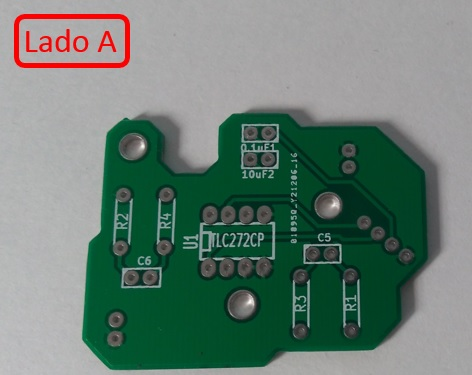
\includegraphics[width=\linewidth]{Figuras/figure_5_a.jpg}
    \center{(a)}
    \end{minipage}%
    \begin{minipage}{0.5\textwidth}
    \centering
    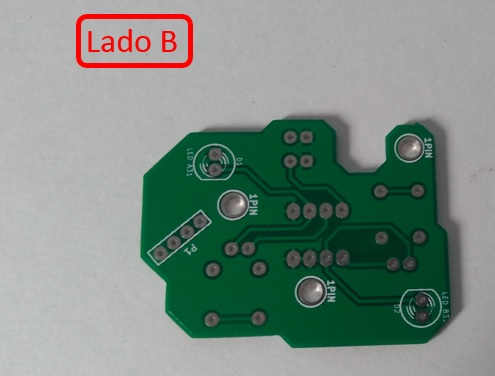
\includegraphics[width=\linewidth]{Figuras/figure_5_b.jpg}   
    \center{(b)}
    \end{minipage}
    \caption{Sensor PCB: (a) Side A, (b) Side B.}
    \label{fig:5}
\end{figure}


\underline{Side A}:

\begin{itemize}
    \item 0.1uF1: Capacitor 0.1 [$\mu$F].
    \item 10uF2: Capacitor 10 [$\mu$F].
    \item R2 y R4: Female pin header 4x1 (Resistances of 1.5 [M$\Omega$]).
    \item R1 y R3: Female pin header 4x1 (Resistances of 10 [M$\Omega$]).
    \item U1 (TLC272CP): TCL272CP Operational Amplifier.
\end{itemize}

\underline{Side B}:

\begin{itemize}
    \item LED A31: Yellow LED.
    \item LED B31: Blue LED.
    \item P1: Male pin header 4x1.
\end{itemize}

Figure \ref{fig:6} shows the aerosol sensor fully assembled. For more constructive details please look at the section \ref{construccion} (Prototype building).


\begin{figure}[H]
   \centering
    \begin{minipage}{.5\textwidth}
    \centering
    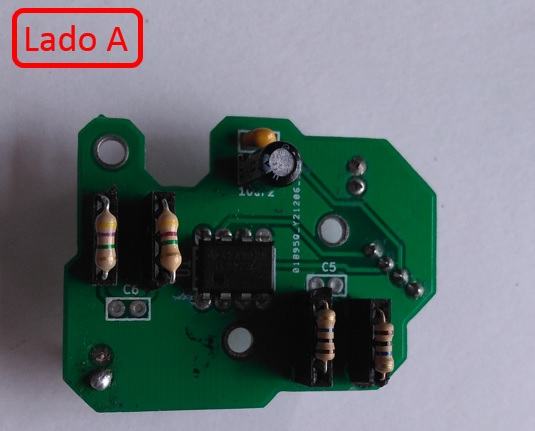
\includegraphics[width=\linewidth]{Figuras/figure_6_a.jpg}
    \center{(a)}
    \end{minipage}%
    \begin{minipage}{0.5\textwidth}
    \centering
    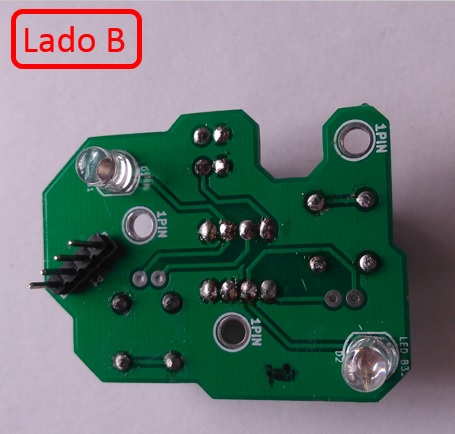
\includegraphics[width=\linewidth]{Figuras/figure_6_b.jpg}   
    \center{(b)}
    \end{minipage}
    \caption{Assembled aerosol sensor: (a) Side A, (b) Side B.}
    \label{fig:6}
\end{figure}

\begin{flushleft}
\textbf{(ii) User interface}
\end{flushleft}

The user interface system contains all the necessary components to interact with the sun photometer. Figure \ref{fig:7} shows its components. The switch (8) of figure \ref{fig:7} is used to turn the Armaduino on and off. The buttons (5) allow the user to choose between the programed functions in the controller board (test mode, measurement and data extraction). The LCD screen (9) is used to provide a visual feedback on the instrument state: (1) Test mode: indicates the measured voltage in the sensors, (2) Measurement: prints the message "measuring" during the data acquisition and then the maximum voltages registered for each sensor at the end of the sample time and (3) Data extraction: prints the message "Extracting data" while the instrument sends the information stored in the memory to the computer.

\begin{figure}[H]
    \centering
    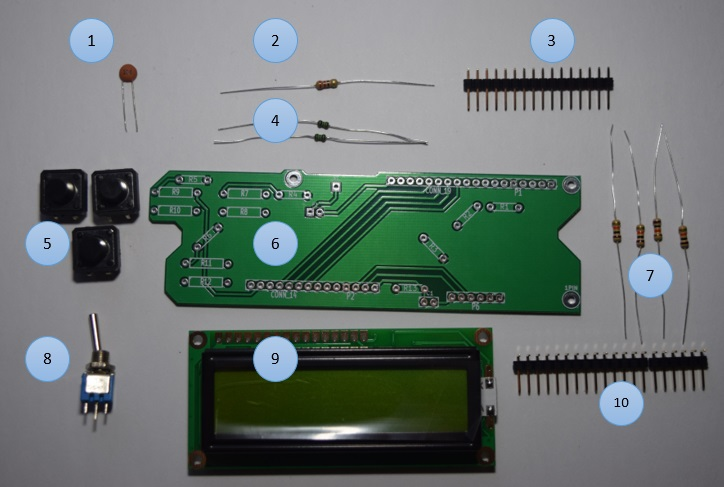
\includegraphics[scale=0.65]{Figuras/figure_7.jpg}
    \caption{User interface components: (1) Capacitor 0.1 [$\mu$F], (2) Resistance 220 [$\Omega$], (3) Male pin header 16x1, (4) Resistances 1 [k$\Omega$], (5) Pushbuttons, (6) Interface PCB, (7) Resistances 10 [k$\Omega$], (8) Switch, (9) LCD screen 16x2, (10) Right angled male pin header 20x1.}
    \label{fig:7}
\end{figure}

Before soldering it is important to separate the right angled male pin header in two parts: one of 14x1 and the other of 6x1 pins. The location of the interface PCB components is described in the next figure, using the board footprints of figure \ref{fig:8} as a reference.

\begin{figure}[H]
    \centering
    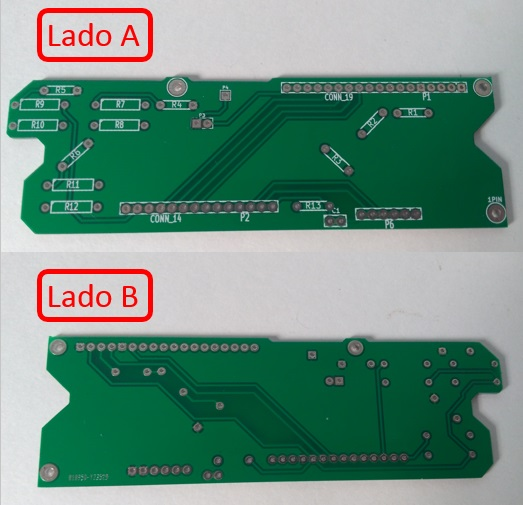
\includegraphics[scale=0.5]{Figuras/figure_8.jpg}
    \caption{Interface PCB faces: (a) Side A, (b) Side B.}
    \label{fig:8}
\end{figure}
%%%% PONER FOTO CON LA PCB POR LOS DOS LADOS %%%%%

\underline{Side A}:

\begin{itemize}
    \item R1 y R2: Resistance of 1 [k$\Omega$].
    \item R3: Resistance of 220 [$\Omega$].
    \item R4, R5, R6 y R13: Resistances of 10 [k$\Omega$].
    \item CONN\_14-P2: Right angled male pin header 14x1.
    \item P6: Rigth angled male pin header 6x1.
    \item C1: Capacitor 0.1 [$\mu$F]
\end{itemize}

\underline{Side B (Footprints on side A)}:

\begin{itemize}
    \item CONN\_19-P1: Male pin header 16x1 soldered to the LCD screen connectors.
    \item R7-R8: Button.
    \item R9-R10: Button.
    \item R11-R12: Button.
\end{itemize}

Figure \ref{fig:9} (a) illustrates how to connect the LCD screen to its corresponding pin headers and figure \ref{fig:9} (b) shows the Armaduino fully assembled. For more details on the construction check section \ref{construccion}.

\begin{figure}[H]
    \centering
    \begin{minipage}{.5\textwidth}
    \centering
    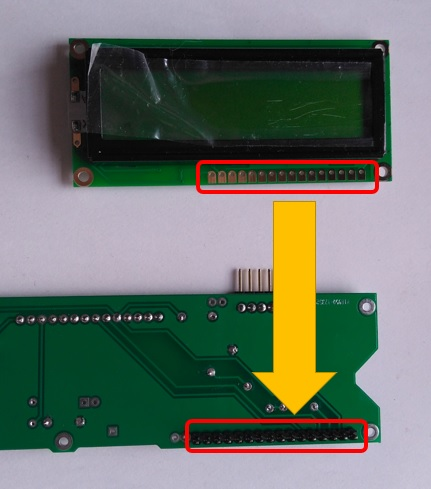
\includegraphics[width=\linewidth]{Figuras/figure_9_b.jpg}
    \center{(a)}
    \end{minipage}%
    \begin{minipage}{0.5\textwidth}
    \centering
    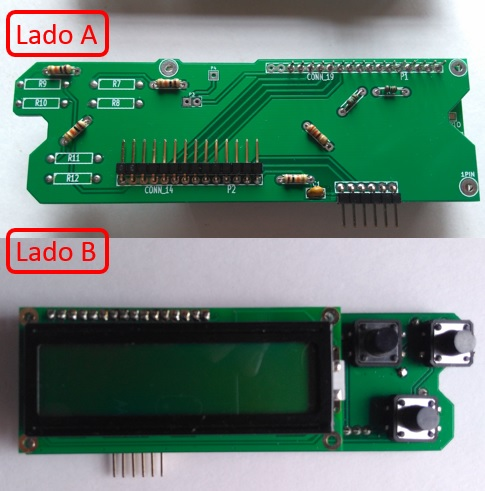
\includegraphics[width=\linewidth]{Figuras/figure_9_a.jpg}   
    \center{(b)}
    \end{minipage}
    \caption{Assembled user interface: (a) Solder the LCD screen to P1 pins, (b) Side A complete (top) and Side B complete (bottom).}
    \label{fig:9}
\end{figure}

% ACA VOY
\begin{flushleft}
\textbf{(iii) Armaduino and Data Logger}
\end{flushleft}

This system is divided in three sub-systems: (1) Armaduino, (2) Data logger, (3) Data logger elements:

\begin{flushleft}
\textbf{(a) Armaduino}
\end{flushleft}

Armaduino is a custom version of the Arduino UNO designed and produced by the chilean company \textit{Ingenieria MCI Ltda}. It is a  prototyping board implemented with the microcontroller ATmega328. As the Arduino UNO, it has 14 digital pins for digital input/output, 6 analog voltage measurement pins and 6 power pins. The main technical reason to use this board instead of the Arduino UNO is that it uses an FTDI port for program loading. Since this port only uses pins already included in the board it enabled an easy way to extend the programming and communication port to the interface panel. This approach does not work with the Arduino UNO because it has some limitations on the external use of the reset pin. Another reason to choose this board is that it increases the educational value of the instrument. Since the components have to be soldered by hand it provides a good oportunity to explain the students the electronic components of a microcontroller board.

The power pins are the following:

\begin{itemize}
    \item VIN: voltage input when the board works with an external power source.
    \item 5V: regulated power source for the microcontroller and other board components.
    \item 3V3: regulated power source of 3.3 [V].
    \item GND: ground pins.
\end{itemize}

Each of the 14 digital pins in Armaduino can be used as input or output with the avaliable functions in the Arduino IDE\footnote{The same programming enviroment used for the Arduino UNO}. This pins operate with a 5 [V] logic and can provide or receive a maximum current of 40 [mA]. Some of this pins have special functions:

\begin{itemize}
    \item Serial (0 (RX) and 1 (TX)): used to receive (RX) and transmit (TX) TTL serial data.
    \item External interrupts (2 y 3): these pins can be configurated to generate or interrupt a process, or to change a variable value.
    \item PWM (3, 5, 6, 9, 10 y 11): can output an 8-bit PWM signal if programmed to do so.
    \item SPI (10 (SS), 11 (MOSI), 12 (MISO), 13 (SCK)): This pins allow SPI communication.
    \item LED (13): in the board there is an incorporated LED connected to the digital pin 13. When the pin is set to HIGH the LED turns on, and when is set to LOW the LED turns off. It is usefull to check if the board is working properly.
\end{itemize}

The 6 analog pins provide a voltage measurement resolution of 10 bits (this is, 1024 different values). By default this pins measure from 0 to 5 [V], being possible to modify this range using the pin AREF. Some of the analog pins also have special functions:

\begin{itemize}
    \item $I^2C$ (4 (SDA) y 5 (SCL)): used for communication $I^2C$ (TWI) with the Wire library.
\end{itemize}

The other board's pins are:

\begin{itemize}
    \item AREF: analog reference voltaje for the analogic inputs.
    \item Reset: can be used to reset the microcontroller (inverse logic).
\end{itemize}

Armaduino components are shown in figure \ref{fig:10}. The location of the components in the armaduino PCB (figure \ref{fig:10} (15)) are easily determined by reading the PCB footprints. Special care has to be put regarding the polarized components orientation (LEDs, diodes, electrolytic capacitors, sockets and ATmega328). These components position is shown in figure \ref{fig:11}.

\begin{figure}[H]
    \centering
    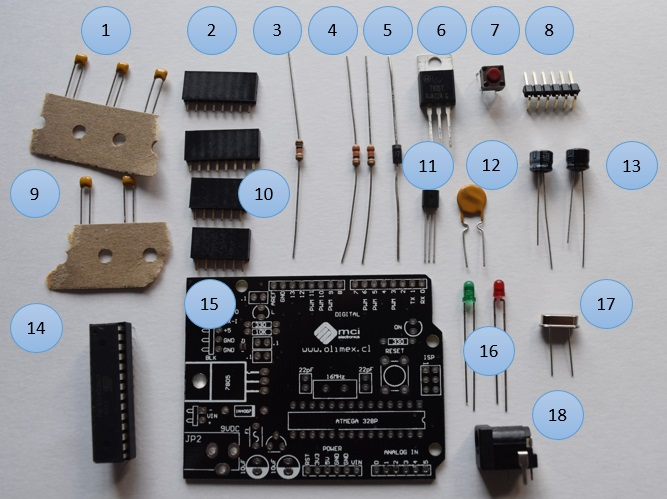
\includegraphics[scale=0.65]{Figuras/figure_10.jpg}
    \caption{Armaduino components: (1) Ceramic Capacitors 0.1 [$\mu$F], (2) Female pin header 8x1, (3) Resistance 10 [k$\Omega$], (4) Resistance 330 [$\Omega$], (5) Diode, (6) Voltage Regulator 5 [V], (7) Mini Push Button, (8) Right angle male pin header, (9) Ceramic capacitors 22 [pF], (10) Female pin headers 6x1, (11) Voltage Regulator 3.3 [V], (12) Fuse, (13) Electrolytic capacitors 10 [$\mu$F], (14) ATmega328 and Socket, (15) Armaduino PCB, (16) Regular LEDs, (17) Crystal oscillator 16 [MHz], (18) Jack power connector.}
    \label{fig:10}
\end{figure}

\begin{figure}[H]
    \centering
    \begin{minipage}{.5\textwidth}
    \centering
    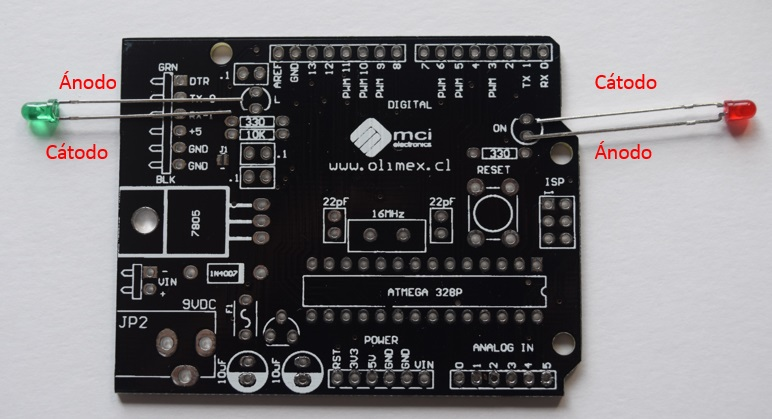
\includegraphics[width=\linewidth]{Figuras/figure_11_a.jpg}
    \center{(a)}
    \end{minipage}%
    \begin{minipage}{0.5\textwidth}
    \centering
    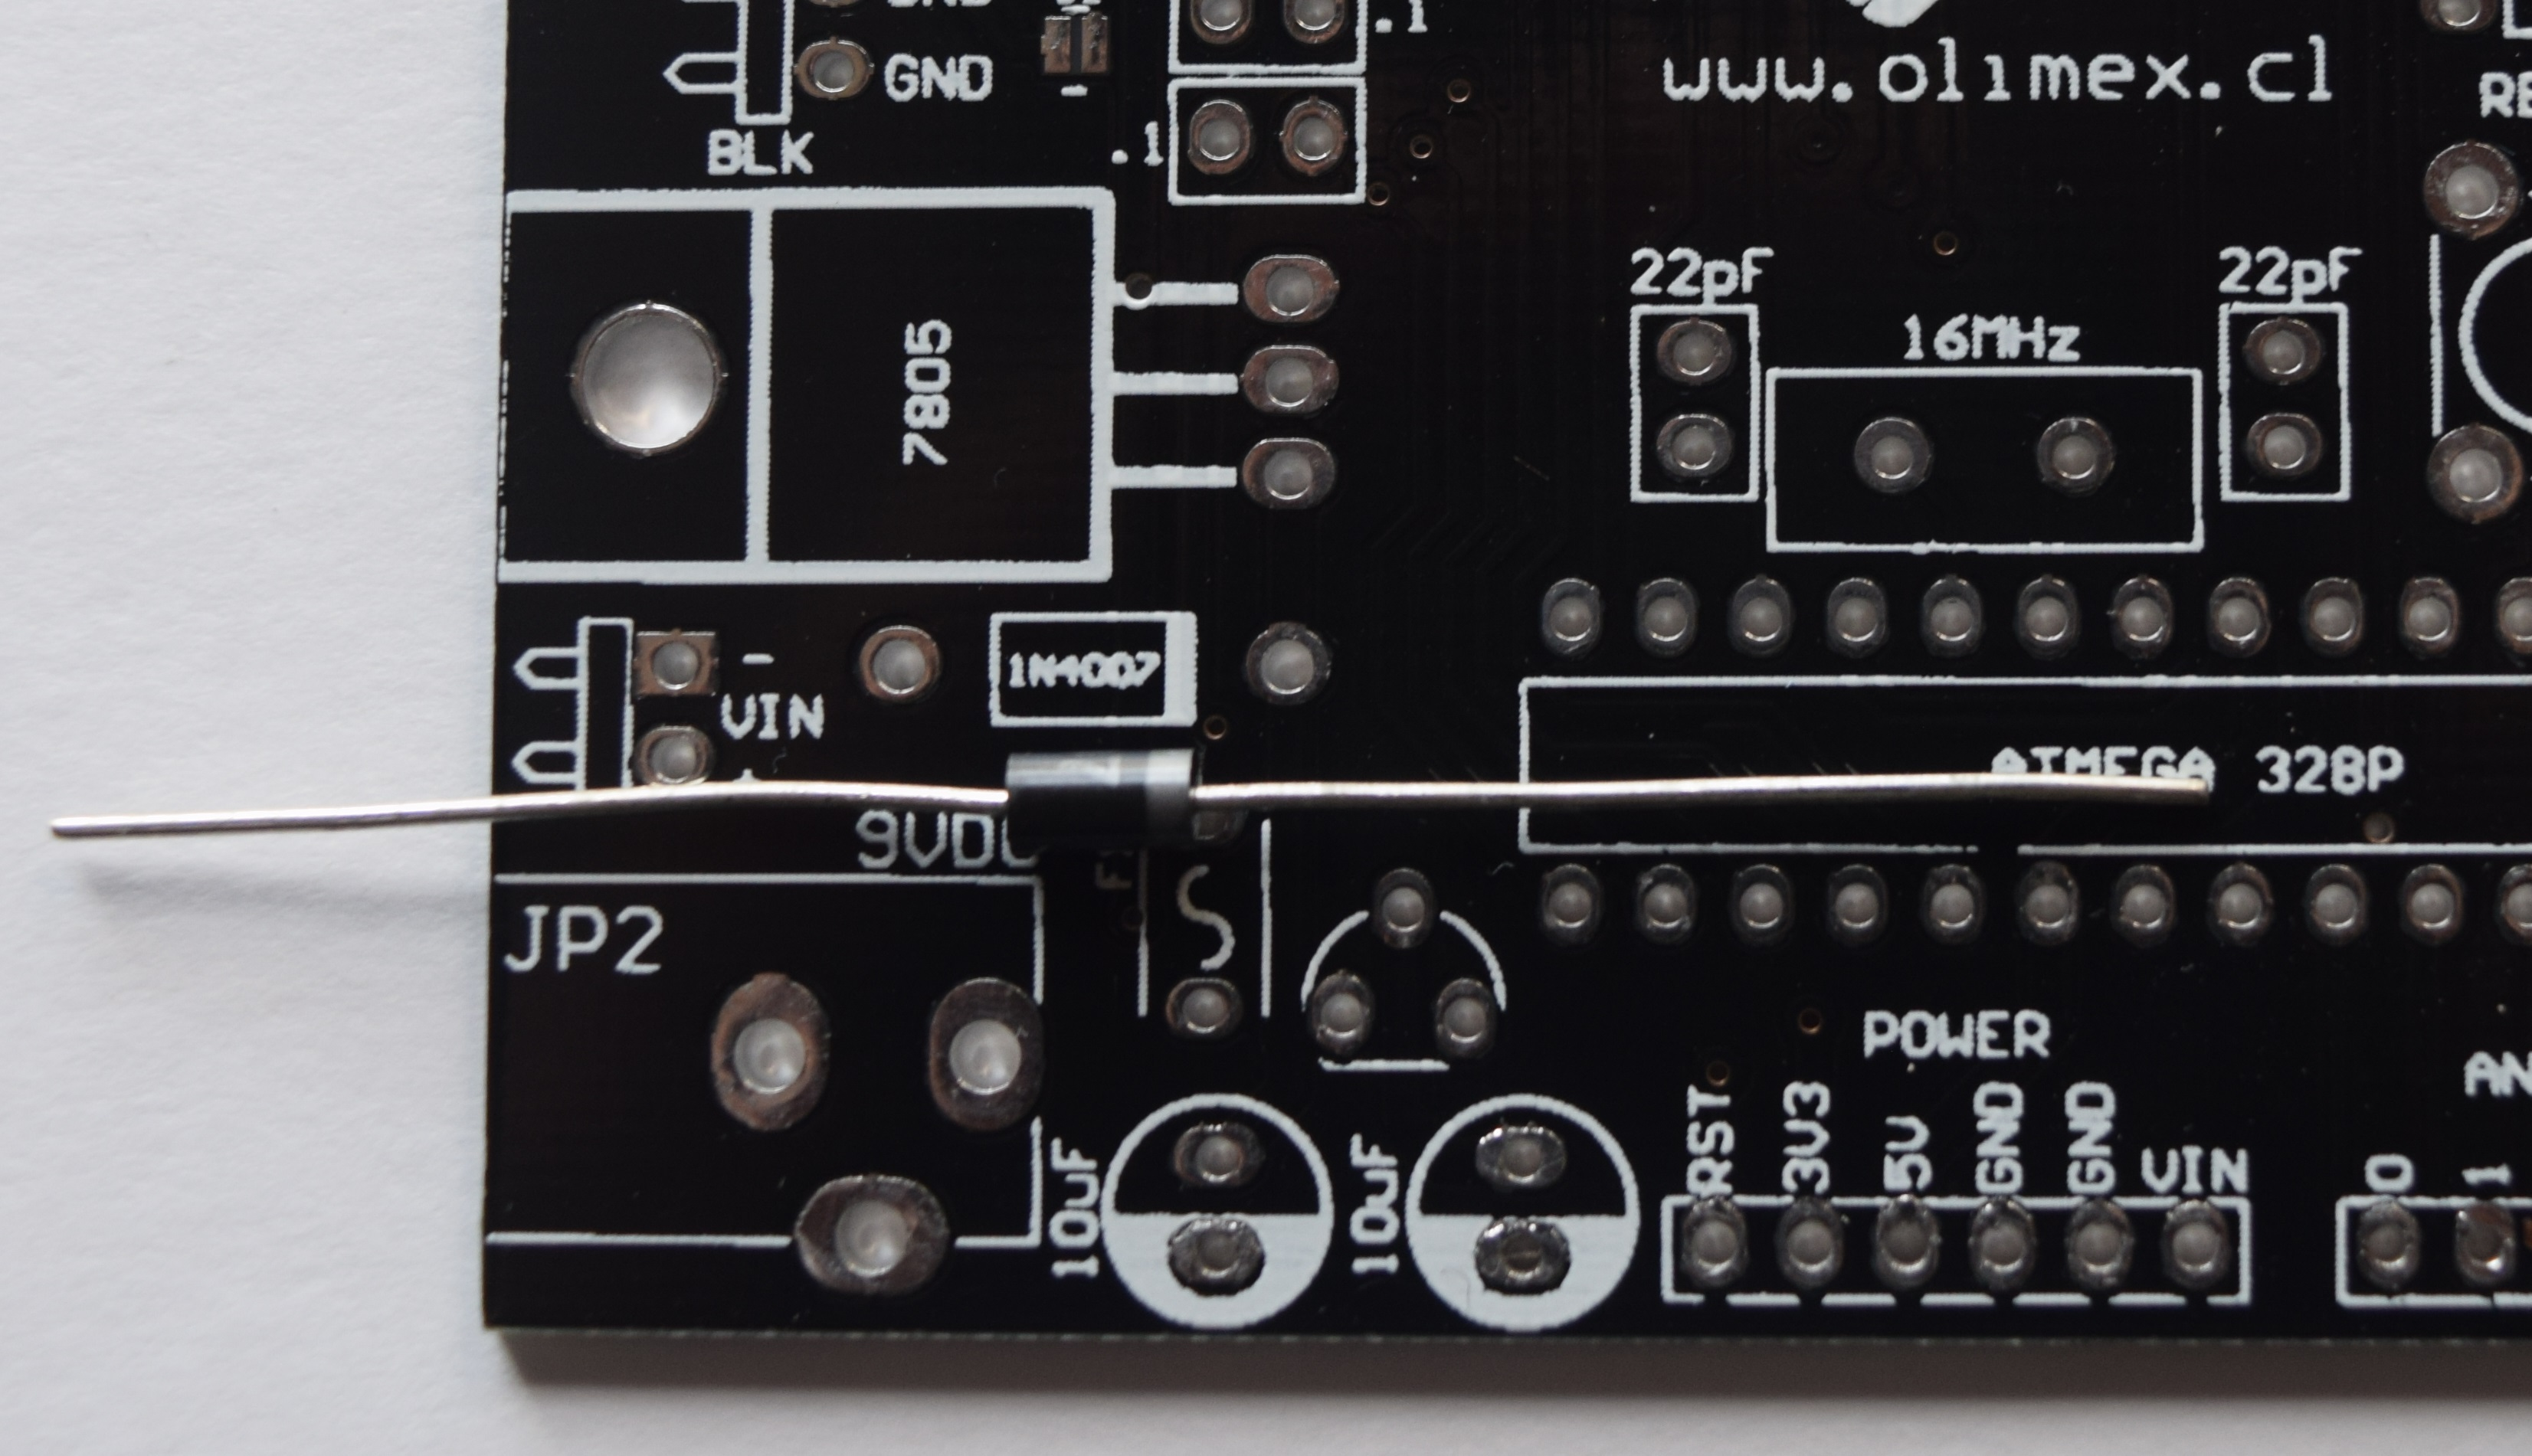
\includegraphics[width=\linewidth]{Figuras/figure_11_b.jpg}   
    \center{(b)}
    \end{minipage}
    \centering
    \begin{minipage}{0.5\textwidth}
    \centering
    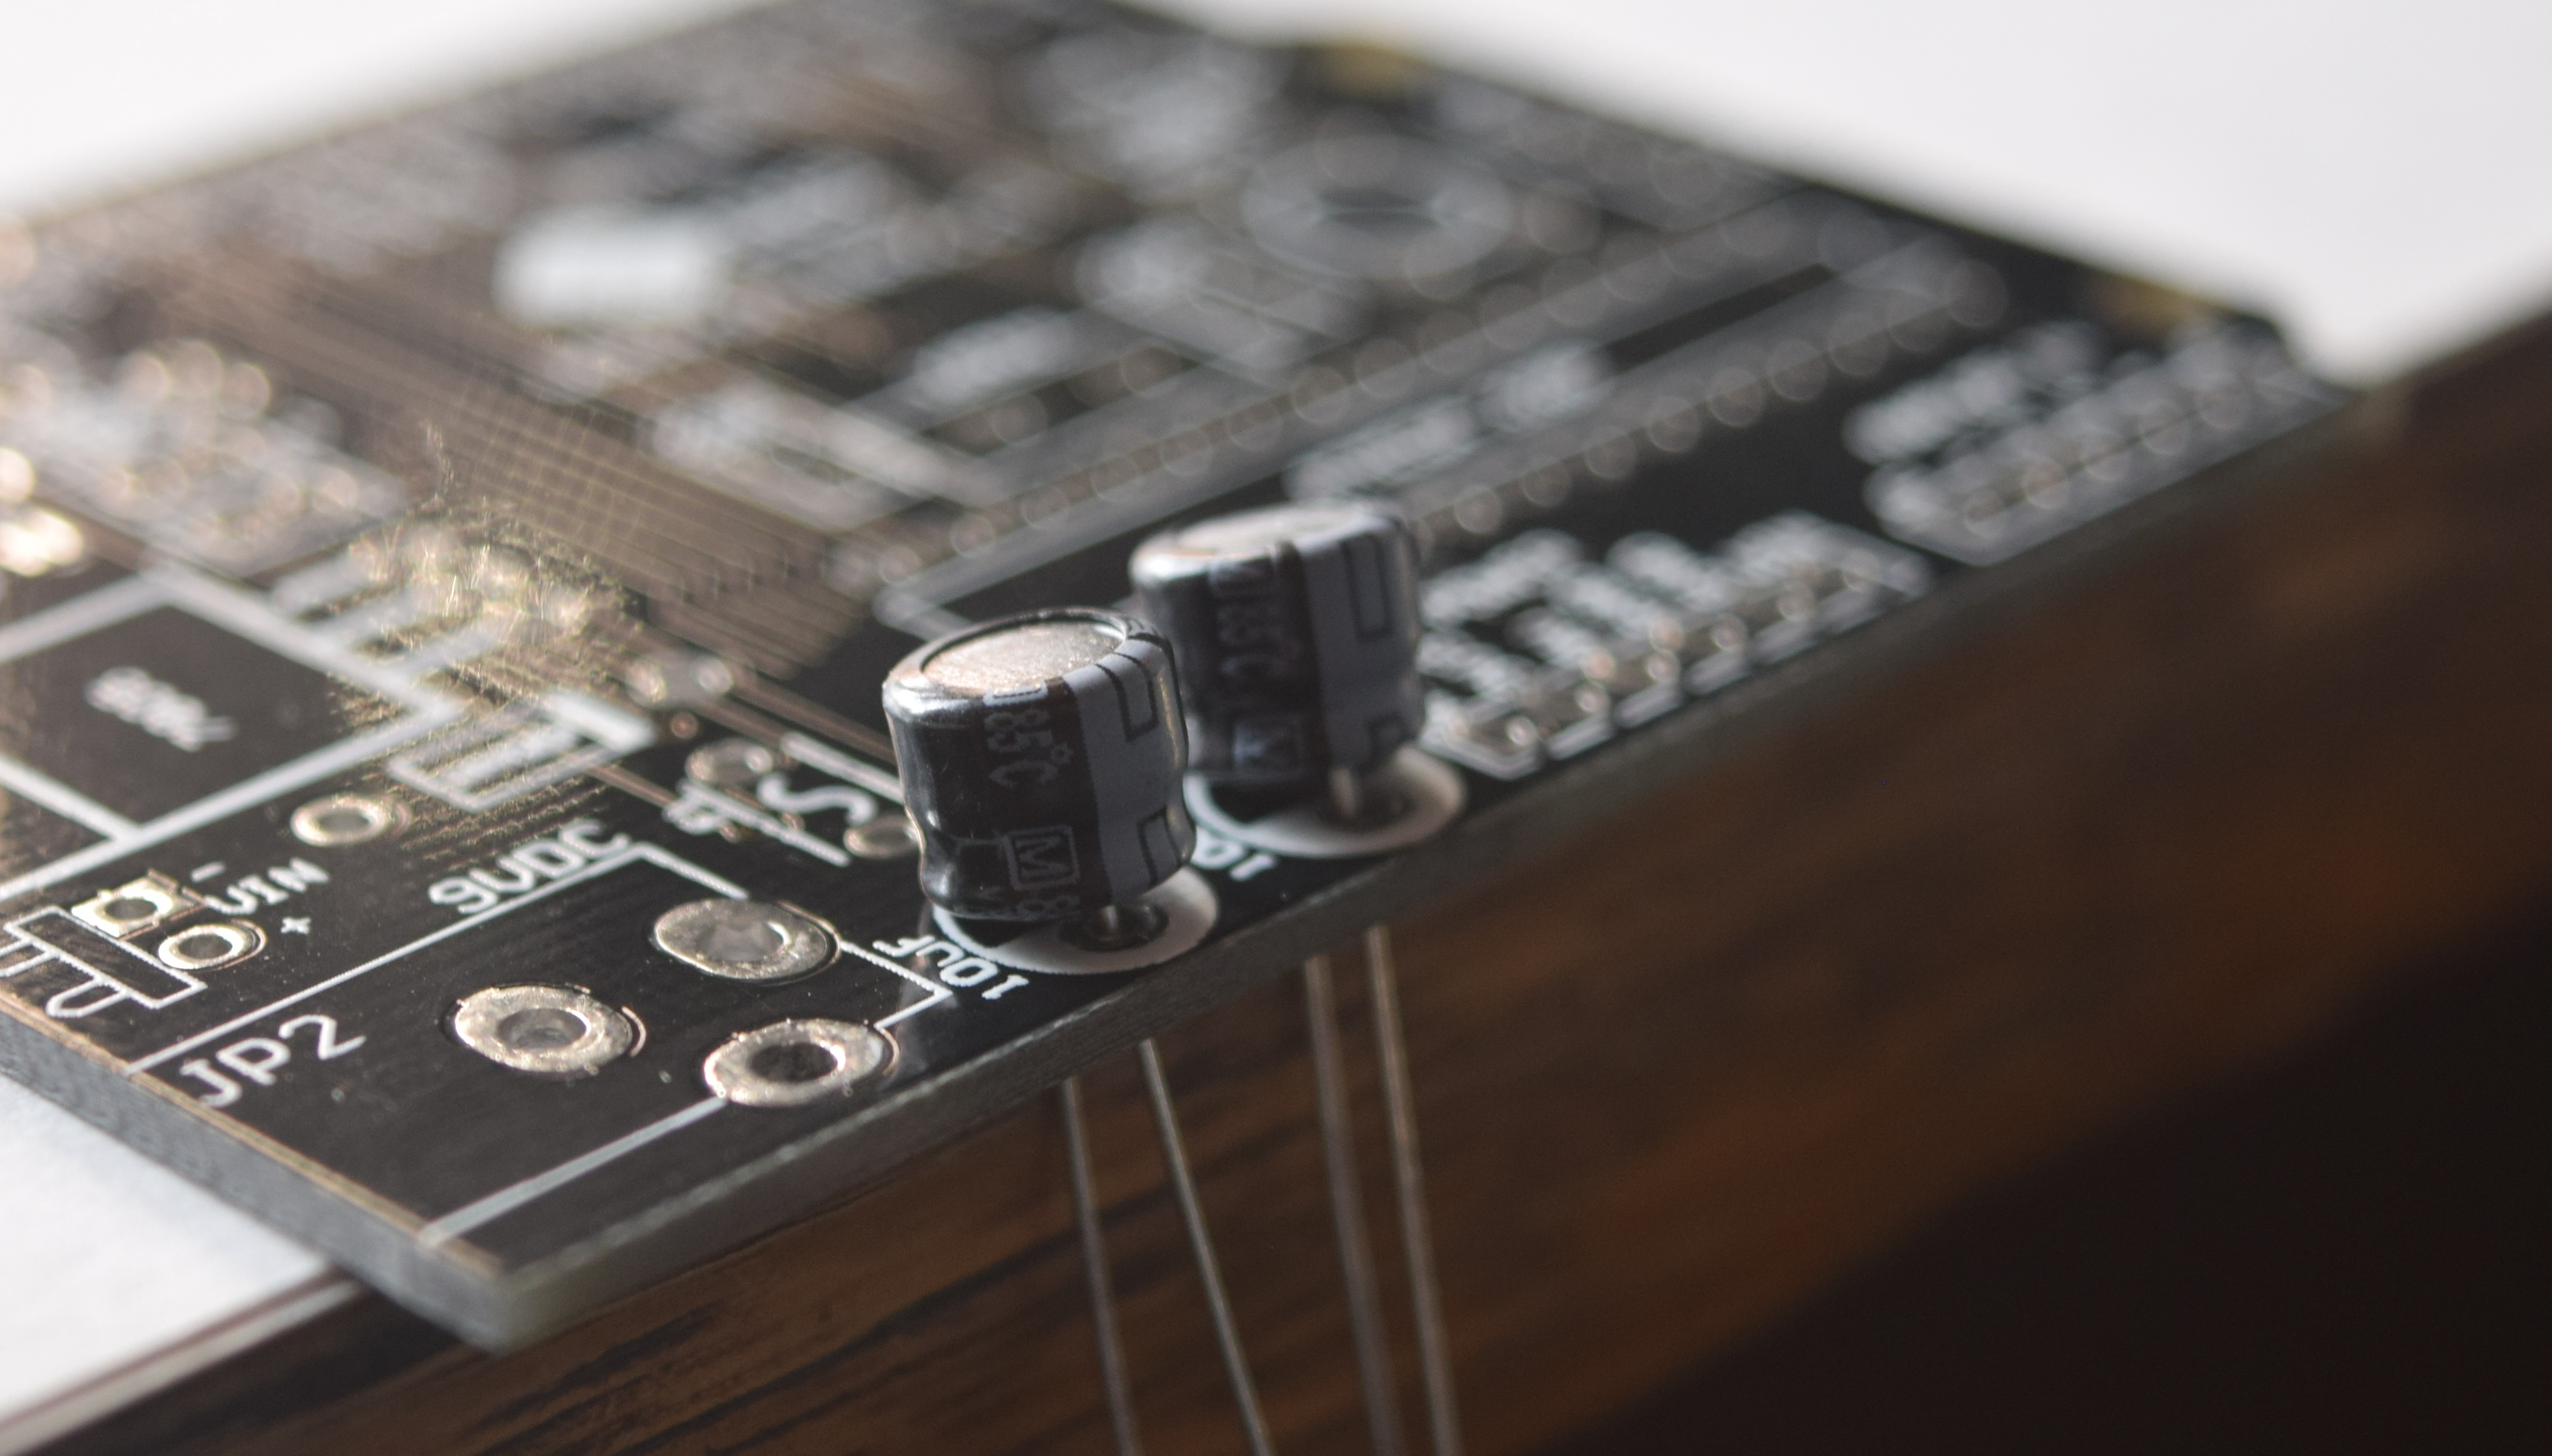
\includegraphics[width=\linewidth]{Figuras/figure_11_c.jpg}
    \center{(c)}
    \end{minipage}%
    \begin{minipage}{0.5\textwidth}
    \centering
    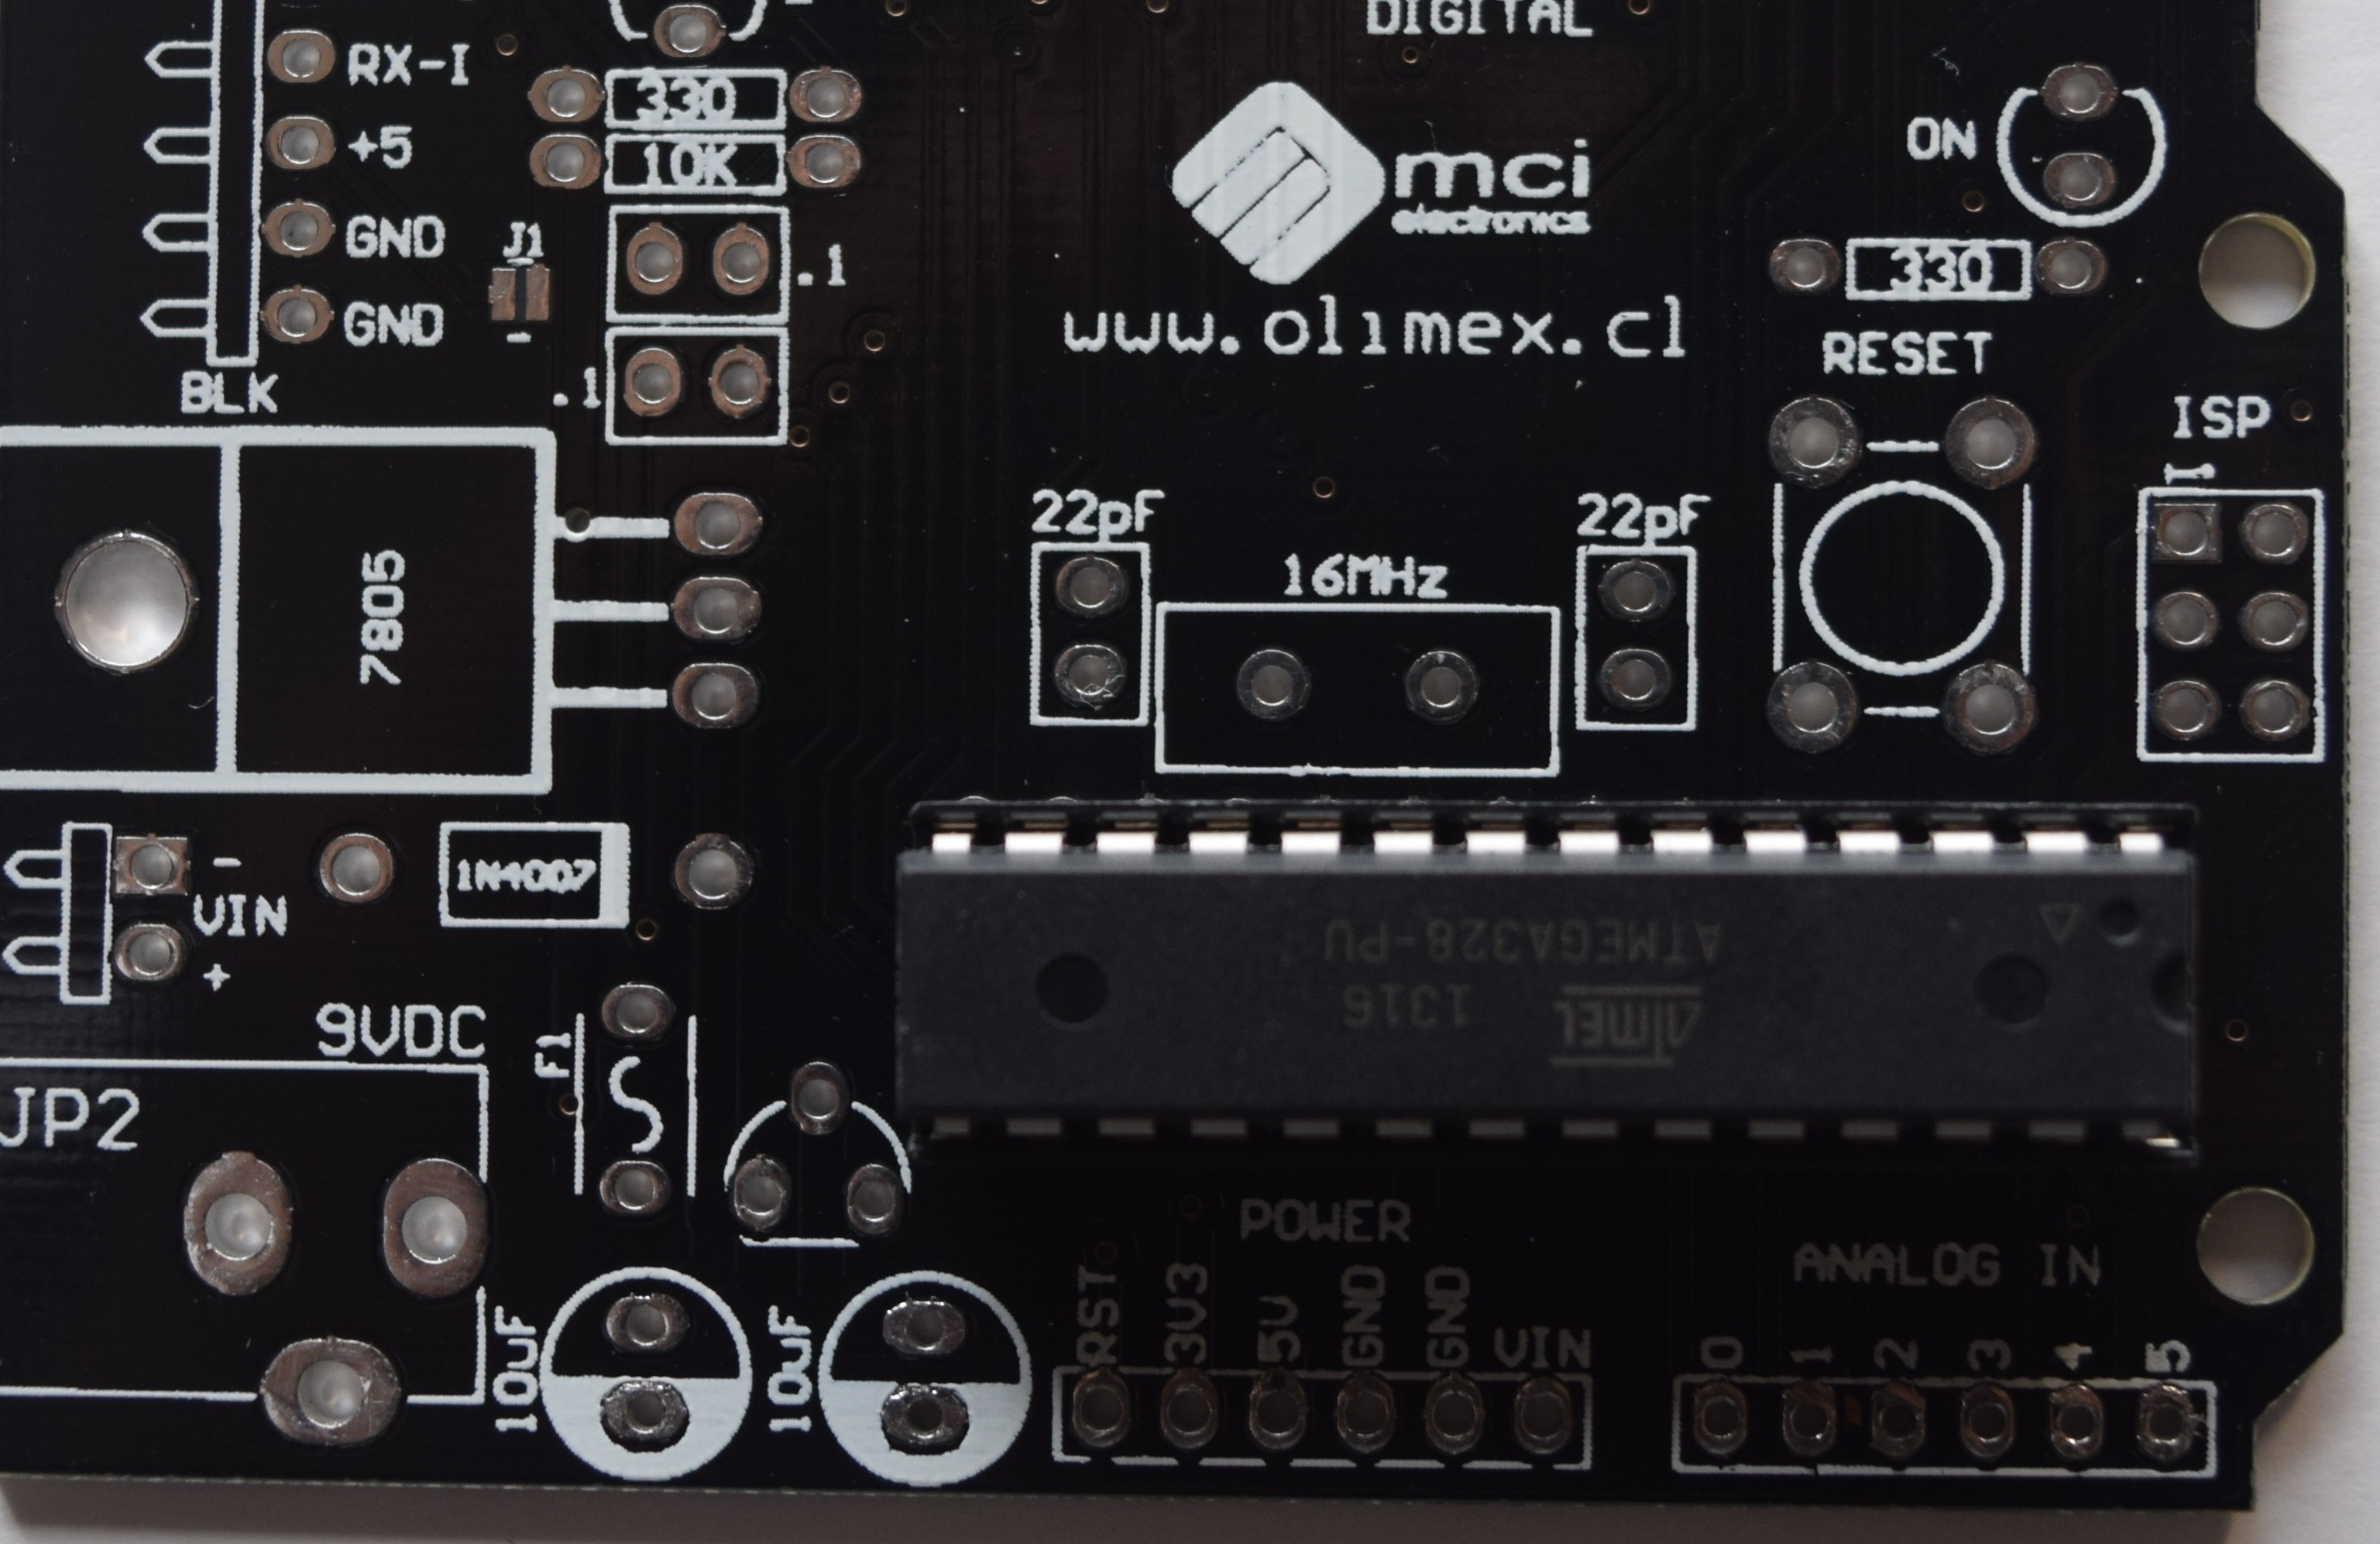
\includegraphics[width=\linewidth]{Figuras/figure_11_d.jpg}   
    \center{(d)}
    \end{minipage}

    \caption{Polarized components position: (a) LEDs, (b) Diode, (c) Electrolytic capacitors and (d) Socket and Atmega328.}
    \label{fig:11}
\end{figure}

Figure \ref{fig:12} shows the armaduino completelly assembled. For more details on the construction go to the section \ref{construccion}: Prototipe building.

\begin{figure}[H]
    \centering
    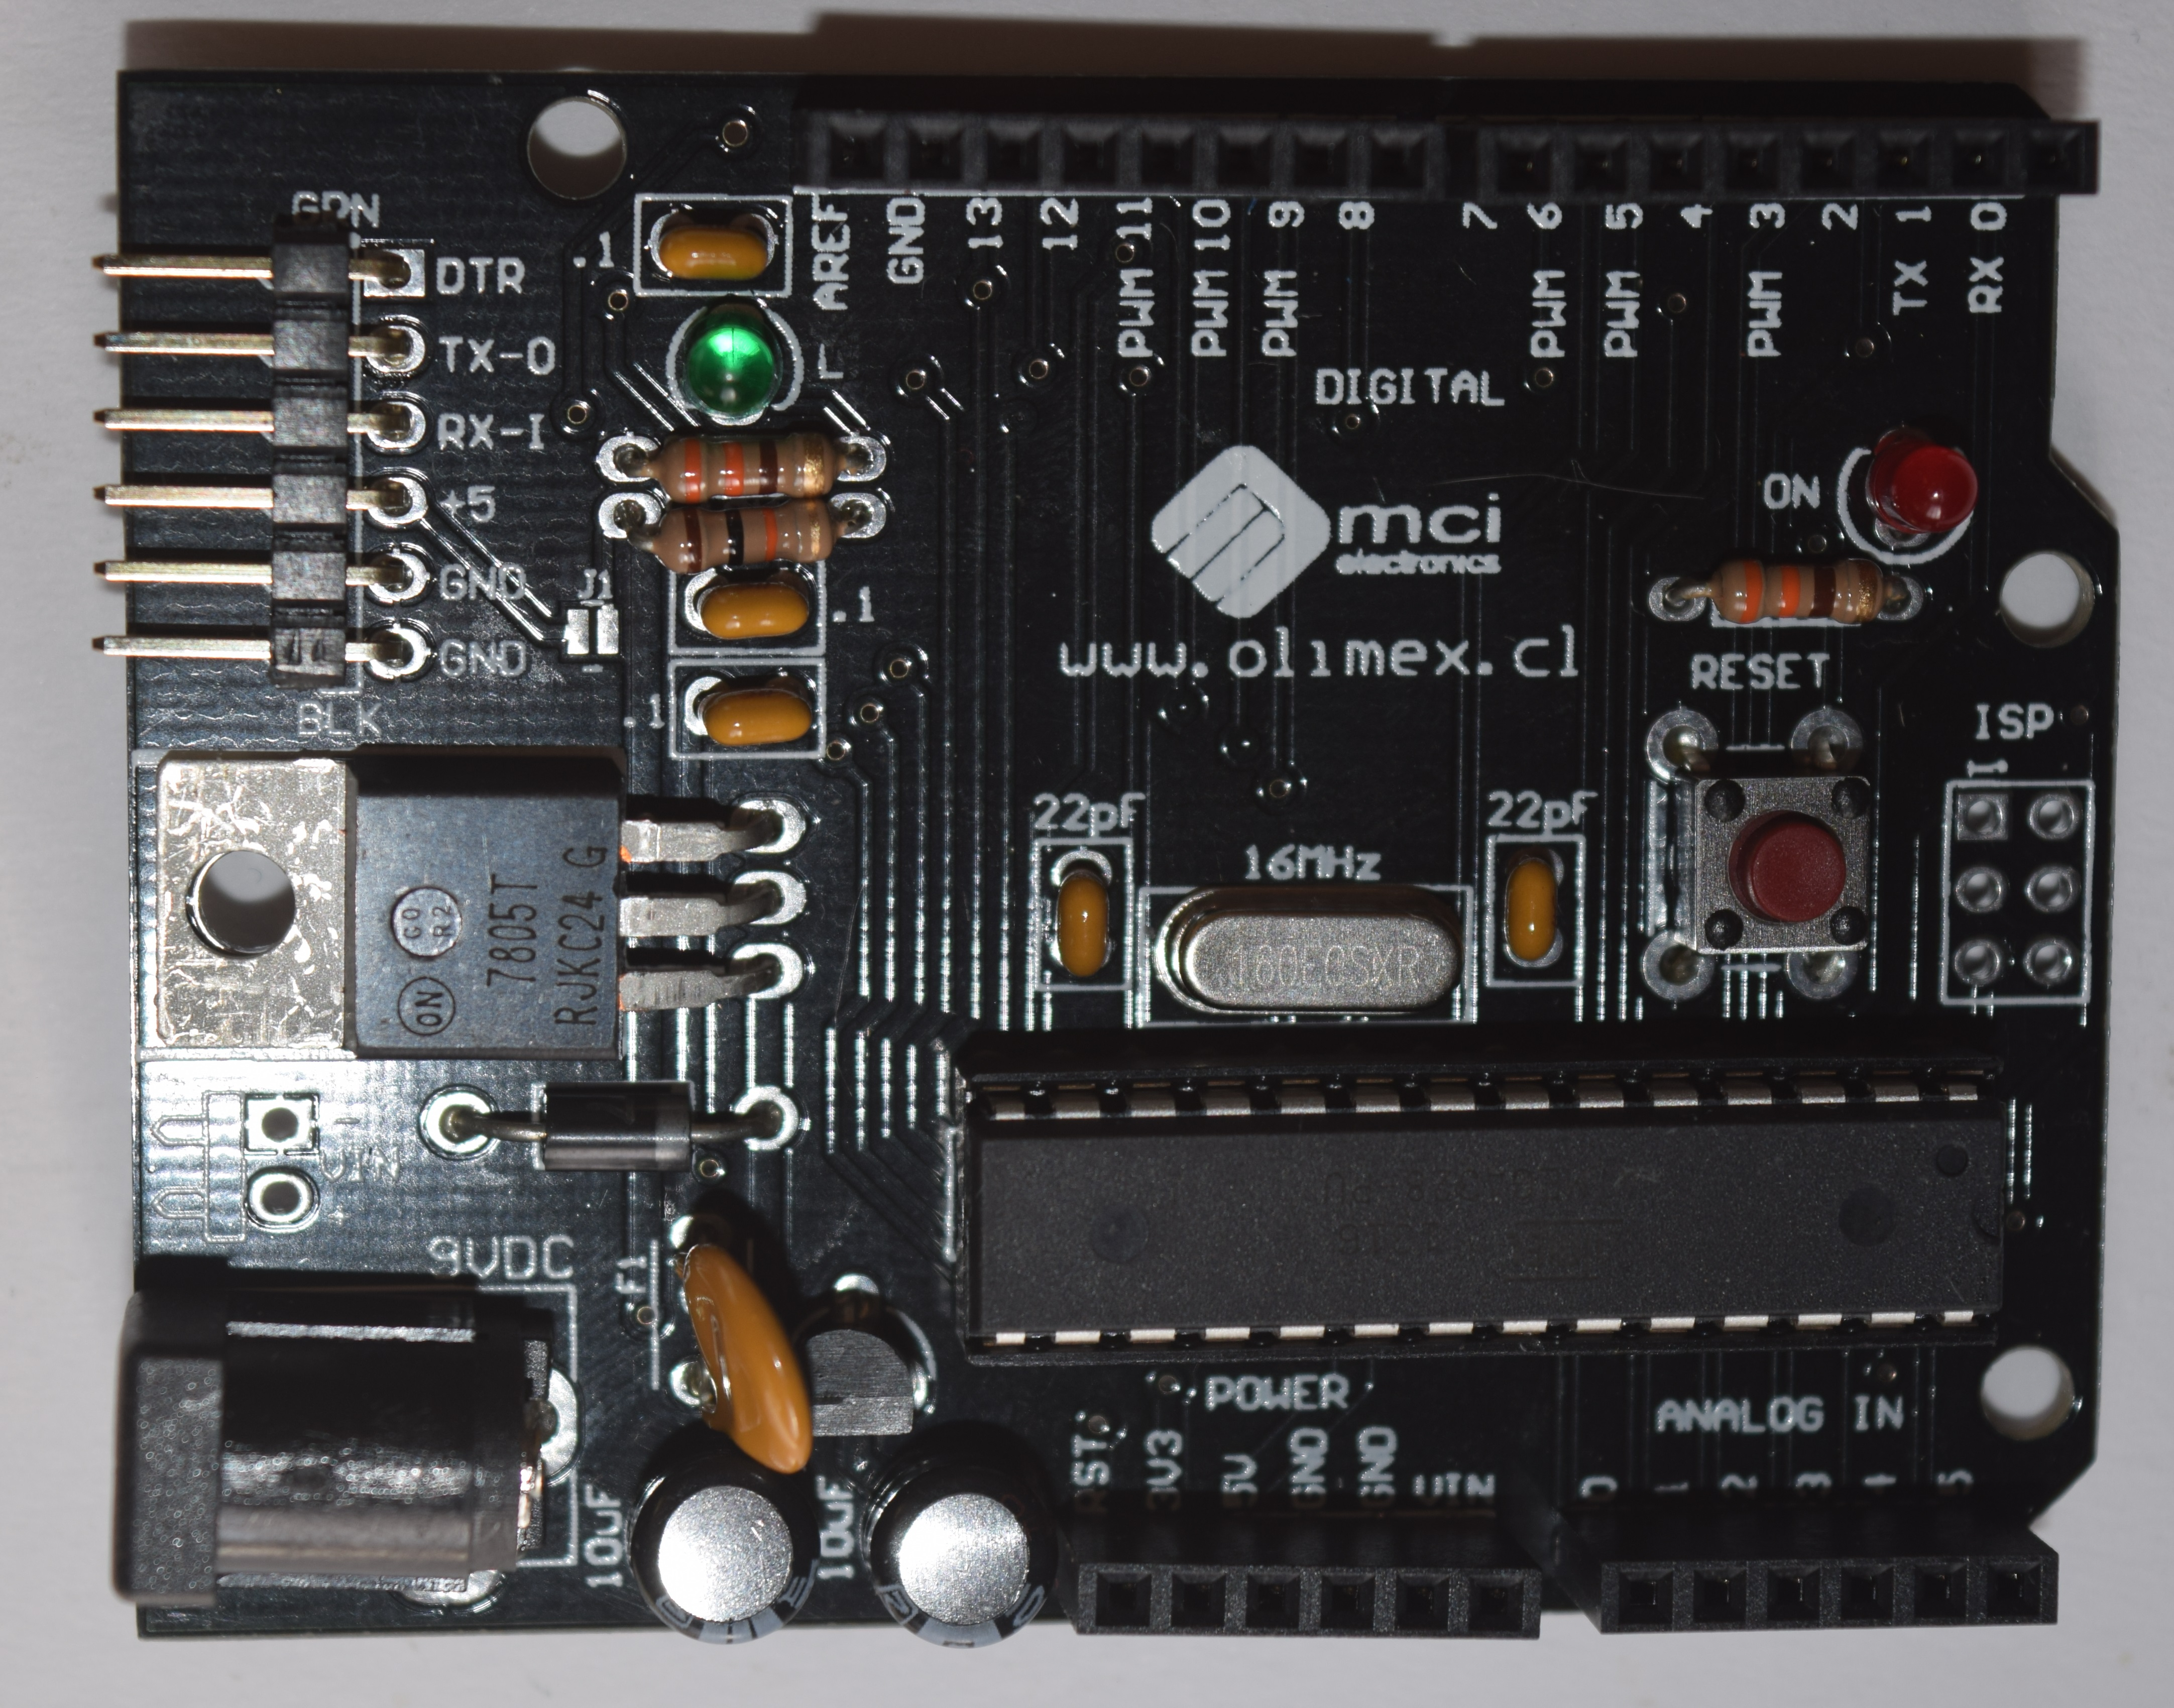
\includegraphics[scale=0.07]{Figuras/figure_12.jpg}
    \caption{Assembled Armaduino.}
    \label{fig:12}
\end{figure}

\begin{flushleft}
\textbf{(b) Data Logger}
\end{flushleft}

The data logger, shown in figure \ref{fig:13}, is a shield board that provides the possibility of storing data in a micro SD (figure \ref{fig:13} (6)). It is composed by a micro SD connector, a reset button and a mesh of 13x12 pin holes separated by 0.1'' for through hole components mounting. In addition it includes a real time clock (RTC) and its battery socket (figure \ref{fig:13} (7)) to enable the storing of the date and time of measurement. The battery enables the conservation of the clock time even when the Armaduino is not connected to a power source. This board is used to register events with an associated timestamp in a file inside the SD, depending on the Armaduino software configuration. Finally, the shield uses the digital pins 6, 8, 11, 12, 13, the analog pins 4, 5 and the reset signal of the Arduino.

\begin{figure}[H]
    \centering
    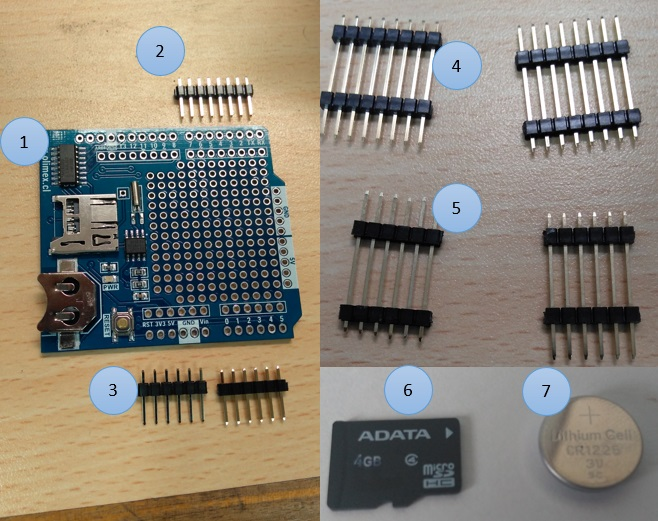
\includegraphics[scale=0.5]{Figuras/figure_13.jpg}
    \caption{Data logger components: (1) Data logger board, (2) Male pin headers 8x1, (3) Male pin headers 6x1, (4) Long male pin headers 8x1, (5) Long male pin headers 6x2, (6) MicroSD card, (7) CR1225 12mm battery.}
    \label{fig:13}
\end{figure}

Figure \ref{fig:14} shows the location of the male pin headers in the data logger board (figure \ref{fig:13} (1)). Male pin headers (figure \ref{fig:14} (b.1) y (b.2)) are used as a board support for the data logger components described in the next section. Long male pin headers (figure \ref{fig:14} (a.1) y (a.2)) are used to mount the datalogger over the Armaduino. Prior to installation of these pins the middle plastic line must be removed in order to leave them as one long pin, as shown in figure \ref{fig:15}. The extracted plastic must be conserved because it will be used for the ensemble of the shield as shown in figure \ref{fig:16} (b). After soldering the pins the removed plastic is placed again in the inferior face of the board.


\begin{figure}[H]
    \centering
    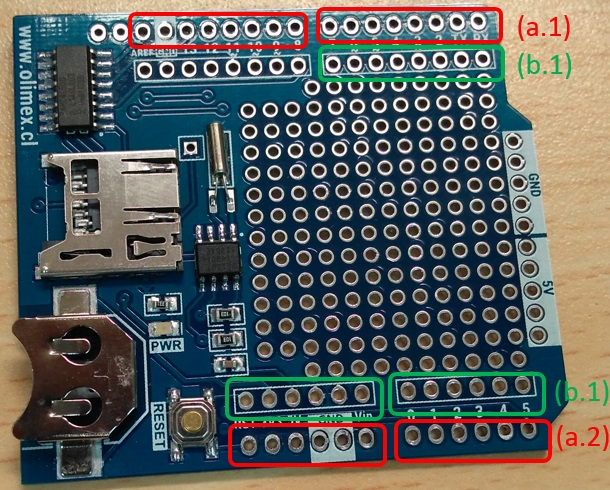
\includegraphics[scale=0.5]{Figuras/figure_14.jpg}
    \caption{Pin location in the data logger board: (a.1) Double male pin headers 8x1, (a.2) Double male pin headers, (b.1) Male pin headers 8x1 and (b.2) Male pin headers 6x1.}
    \label{fig:14}
\end{figure}

\begin{figure}[H]
    \centering
    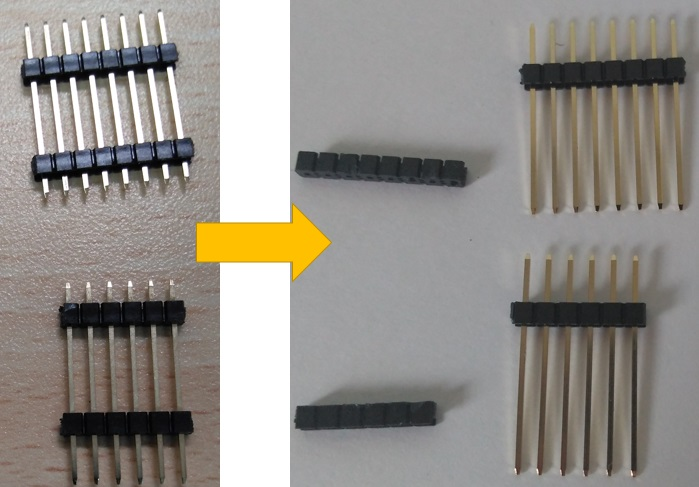
\includegraphics[scale=0.5]{Figuras/figure_15.jpg}
    \caption{Long male pin headers without the middle plastic: Original state (left) and final state (right).}
    \label{fig:15}
\end{figure}

Figure \ref{fig:16} shows the Armaduino assembled. For more building details review section \ref{construccion}.

\begin{figure}[H]
    \centering
    \begin{minipage}{.4\textwidth}
    \centering
    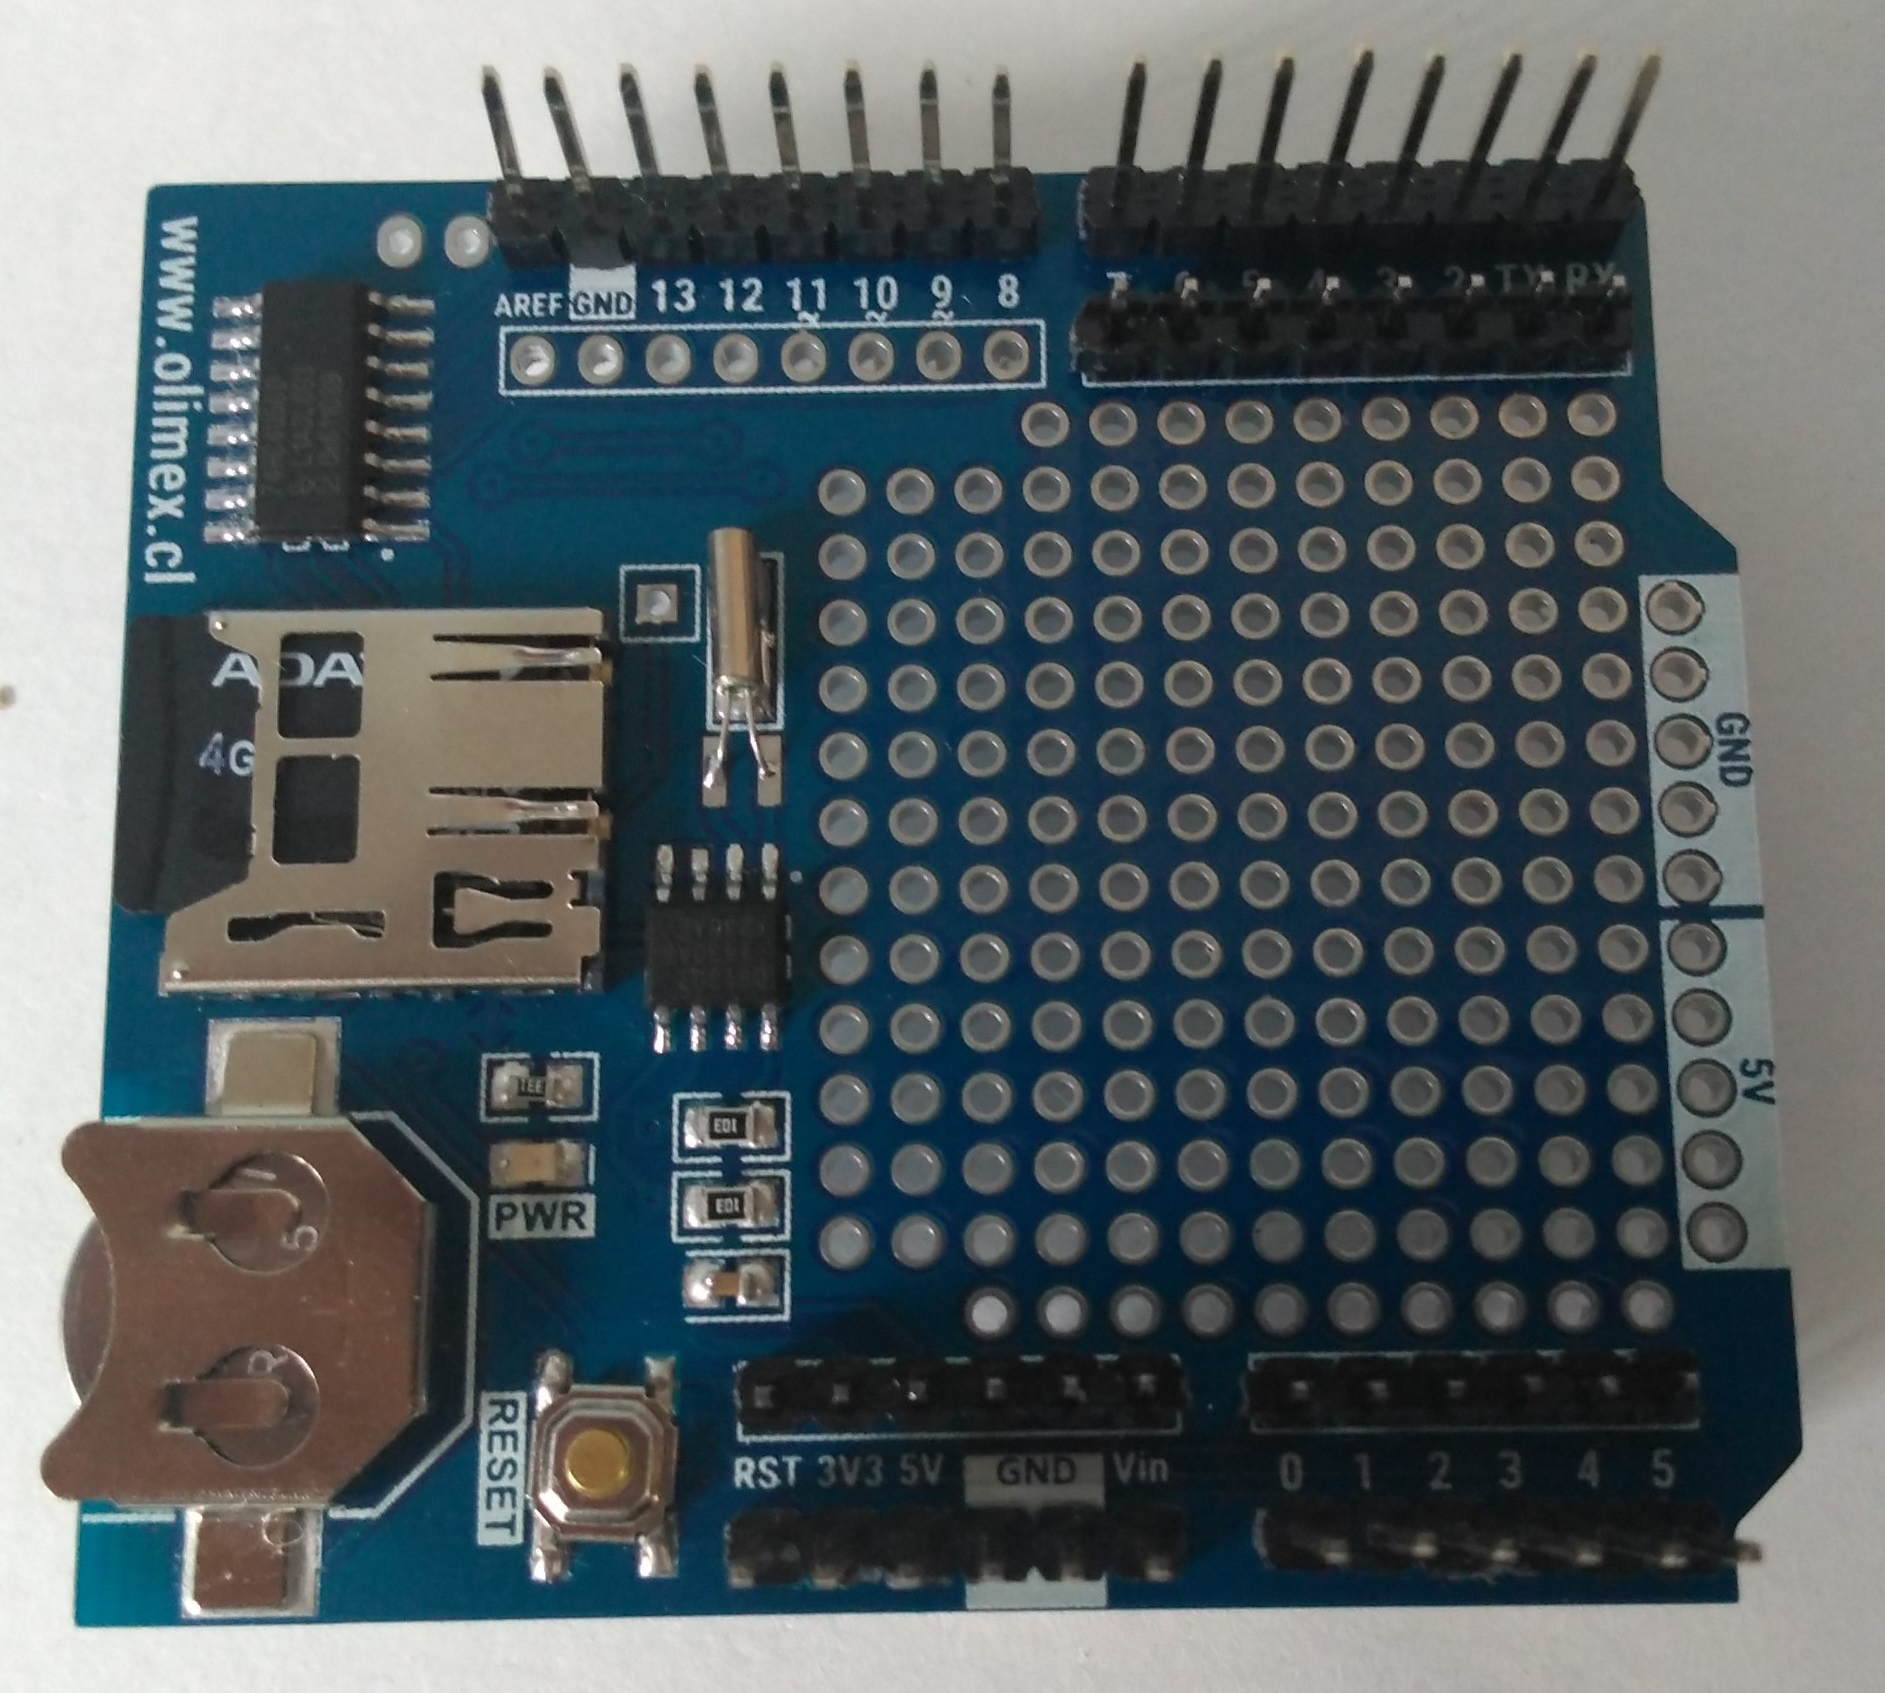
\includegraphics[width=\linewidth]{Figuras/figure_16_a.jpg}
    \center{(a)}
    \end{minipage}
    \centering
    \begin{minipage}{.4\textwidth}
    \centering
    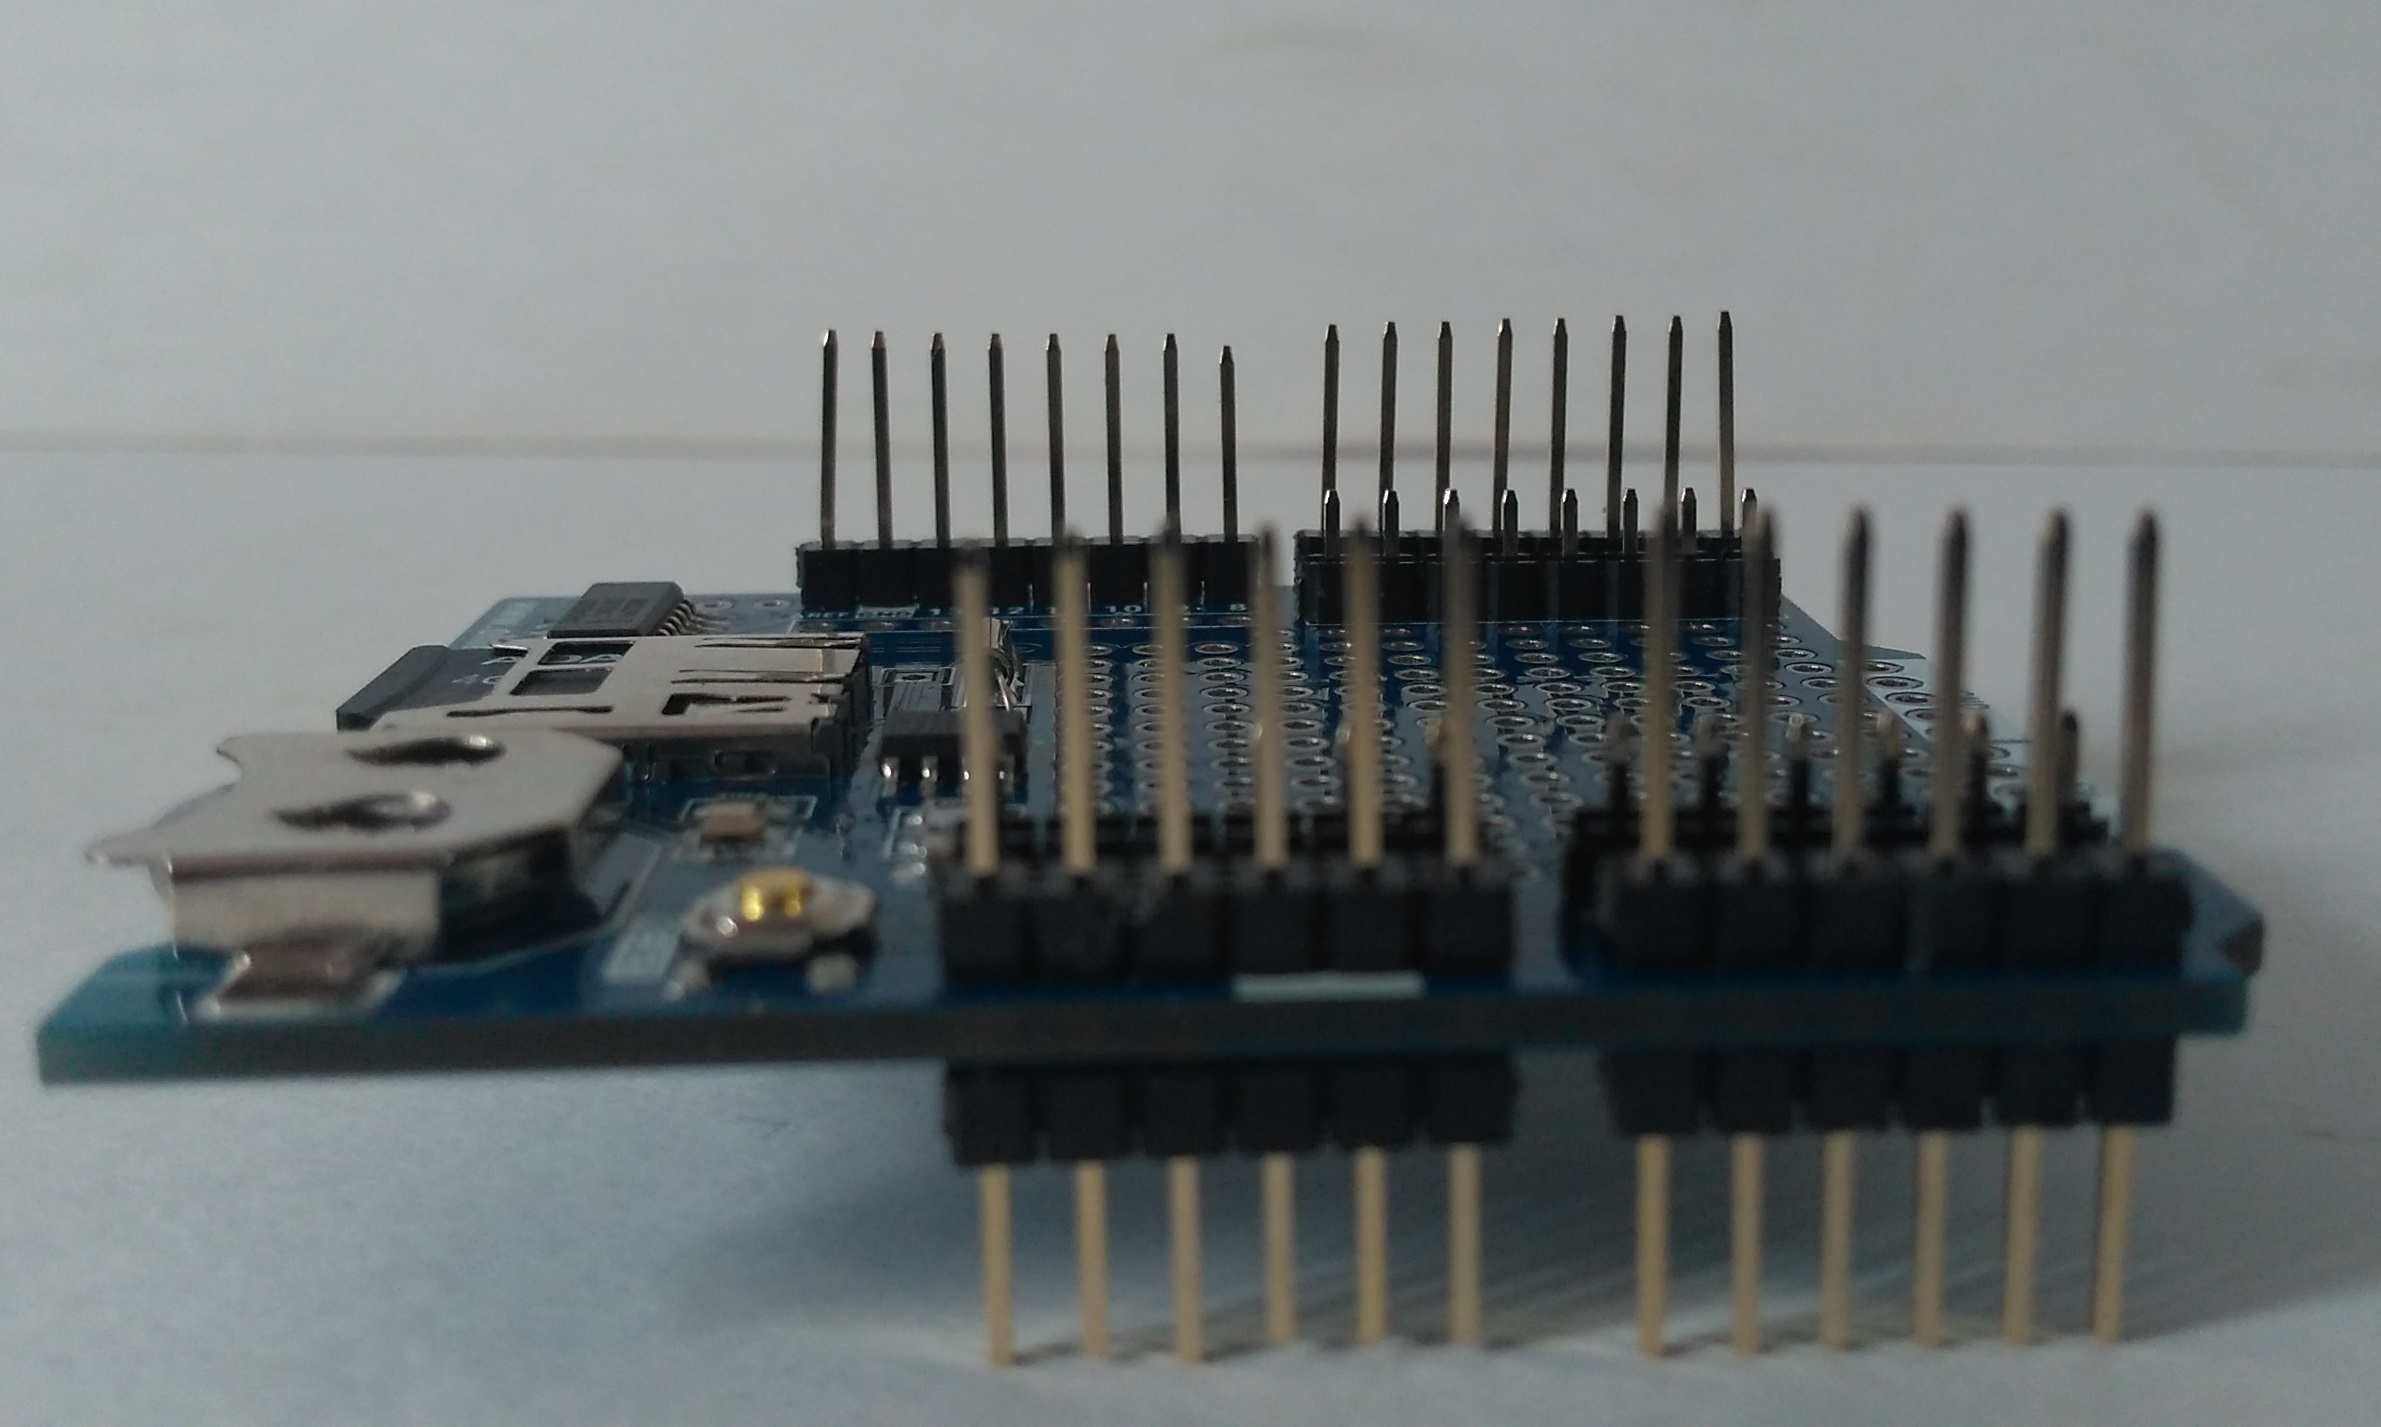
\includegraphics[width=\linewidth]{Figuras/figure_16_b.jpg}
    \center{(b)}
    \end{minipage}
    
    \caption{Assembled data logger:(a) Top view and (b) Side view.}
    \label{fig:16}
\end{figure}


\begin{flushleft}
\textbf{(c) Data Logger mini-board}
\end{flushleft}

This board is used to ease the soldering of components and their connection to the data logger. Figure \ref{fig:17} shows the subsystem components. The male molex macho 4x1 (figure \ref{fig:17} (2)) is used to communicate the aerosol optical sensor with the Armaduino. The male molex 2x1 (figura \ref{fig:17} (6)) is used to provide power the 9V battery power to the Armaduino. The buzzer (figure \ref{fig:17} (5)) emits sound feedback for different use cases of the prototype. Finally, the BMP 180 sensor (figure \ref{fig:17} (4)) is used to measure pressure and temperature at the time of each AOT measurement.

\begin{figure}[H]
    \centering
    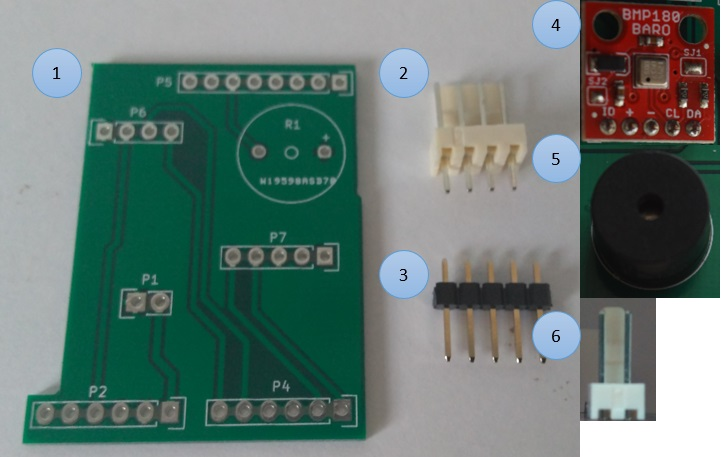
\includegraphics[scale=0.5]{Figuras/figure_17.jpg}
    \caption{Mini-board components: (1) Mini-board, (2) Male Molex 4x1, (3) Male pin header 5x1, (4) BMP180 pressure and temperature sensor, (5) 12mm PCB mountable buzzer 2.048kHz, (6) Male molex 2x1.}
    \label{fig:17}
\end{figure}

Next the location of the components in the mini-board is described. They are refered to the board footprints shown in figure \ref{fig:17} (1).

\begin{itemize}
    \item P6: Male molex 4x1.
    \item R1: Buzzer (watch the + symbol on the buzzer).
    \item P7: Male pin headers 5x1. The BMP180 sensor is mounted here.
    \item P1: Male molex connector 2x1.
\end{itemize}

Figure \ref{fig:18} shows the fully assembled mini-board. For more details on the assembling check section \ref{construccion}.

\begin{figure}[H]
    \centering
    \begin{minipage}{.45\textwidth}
    \centering
    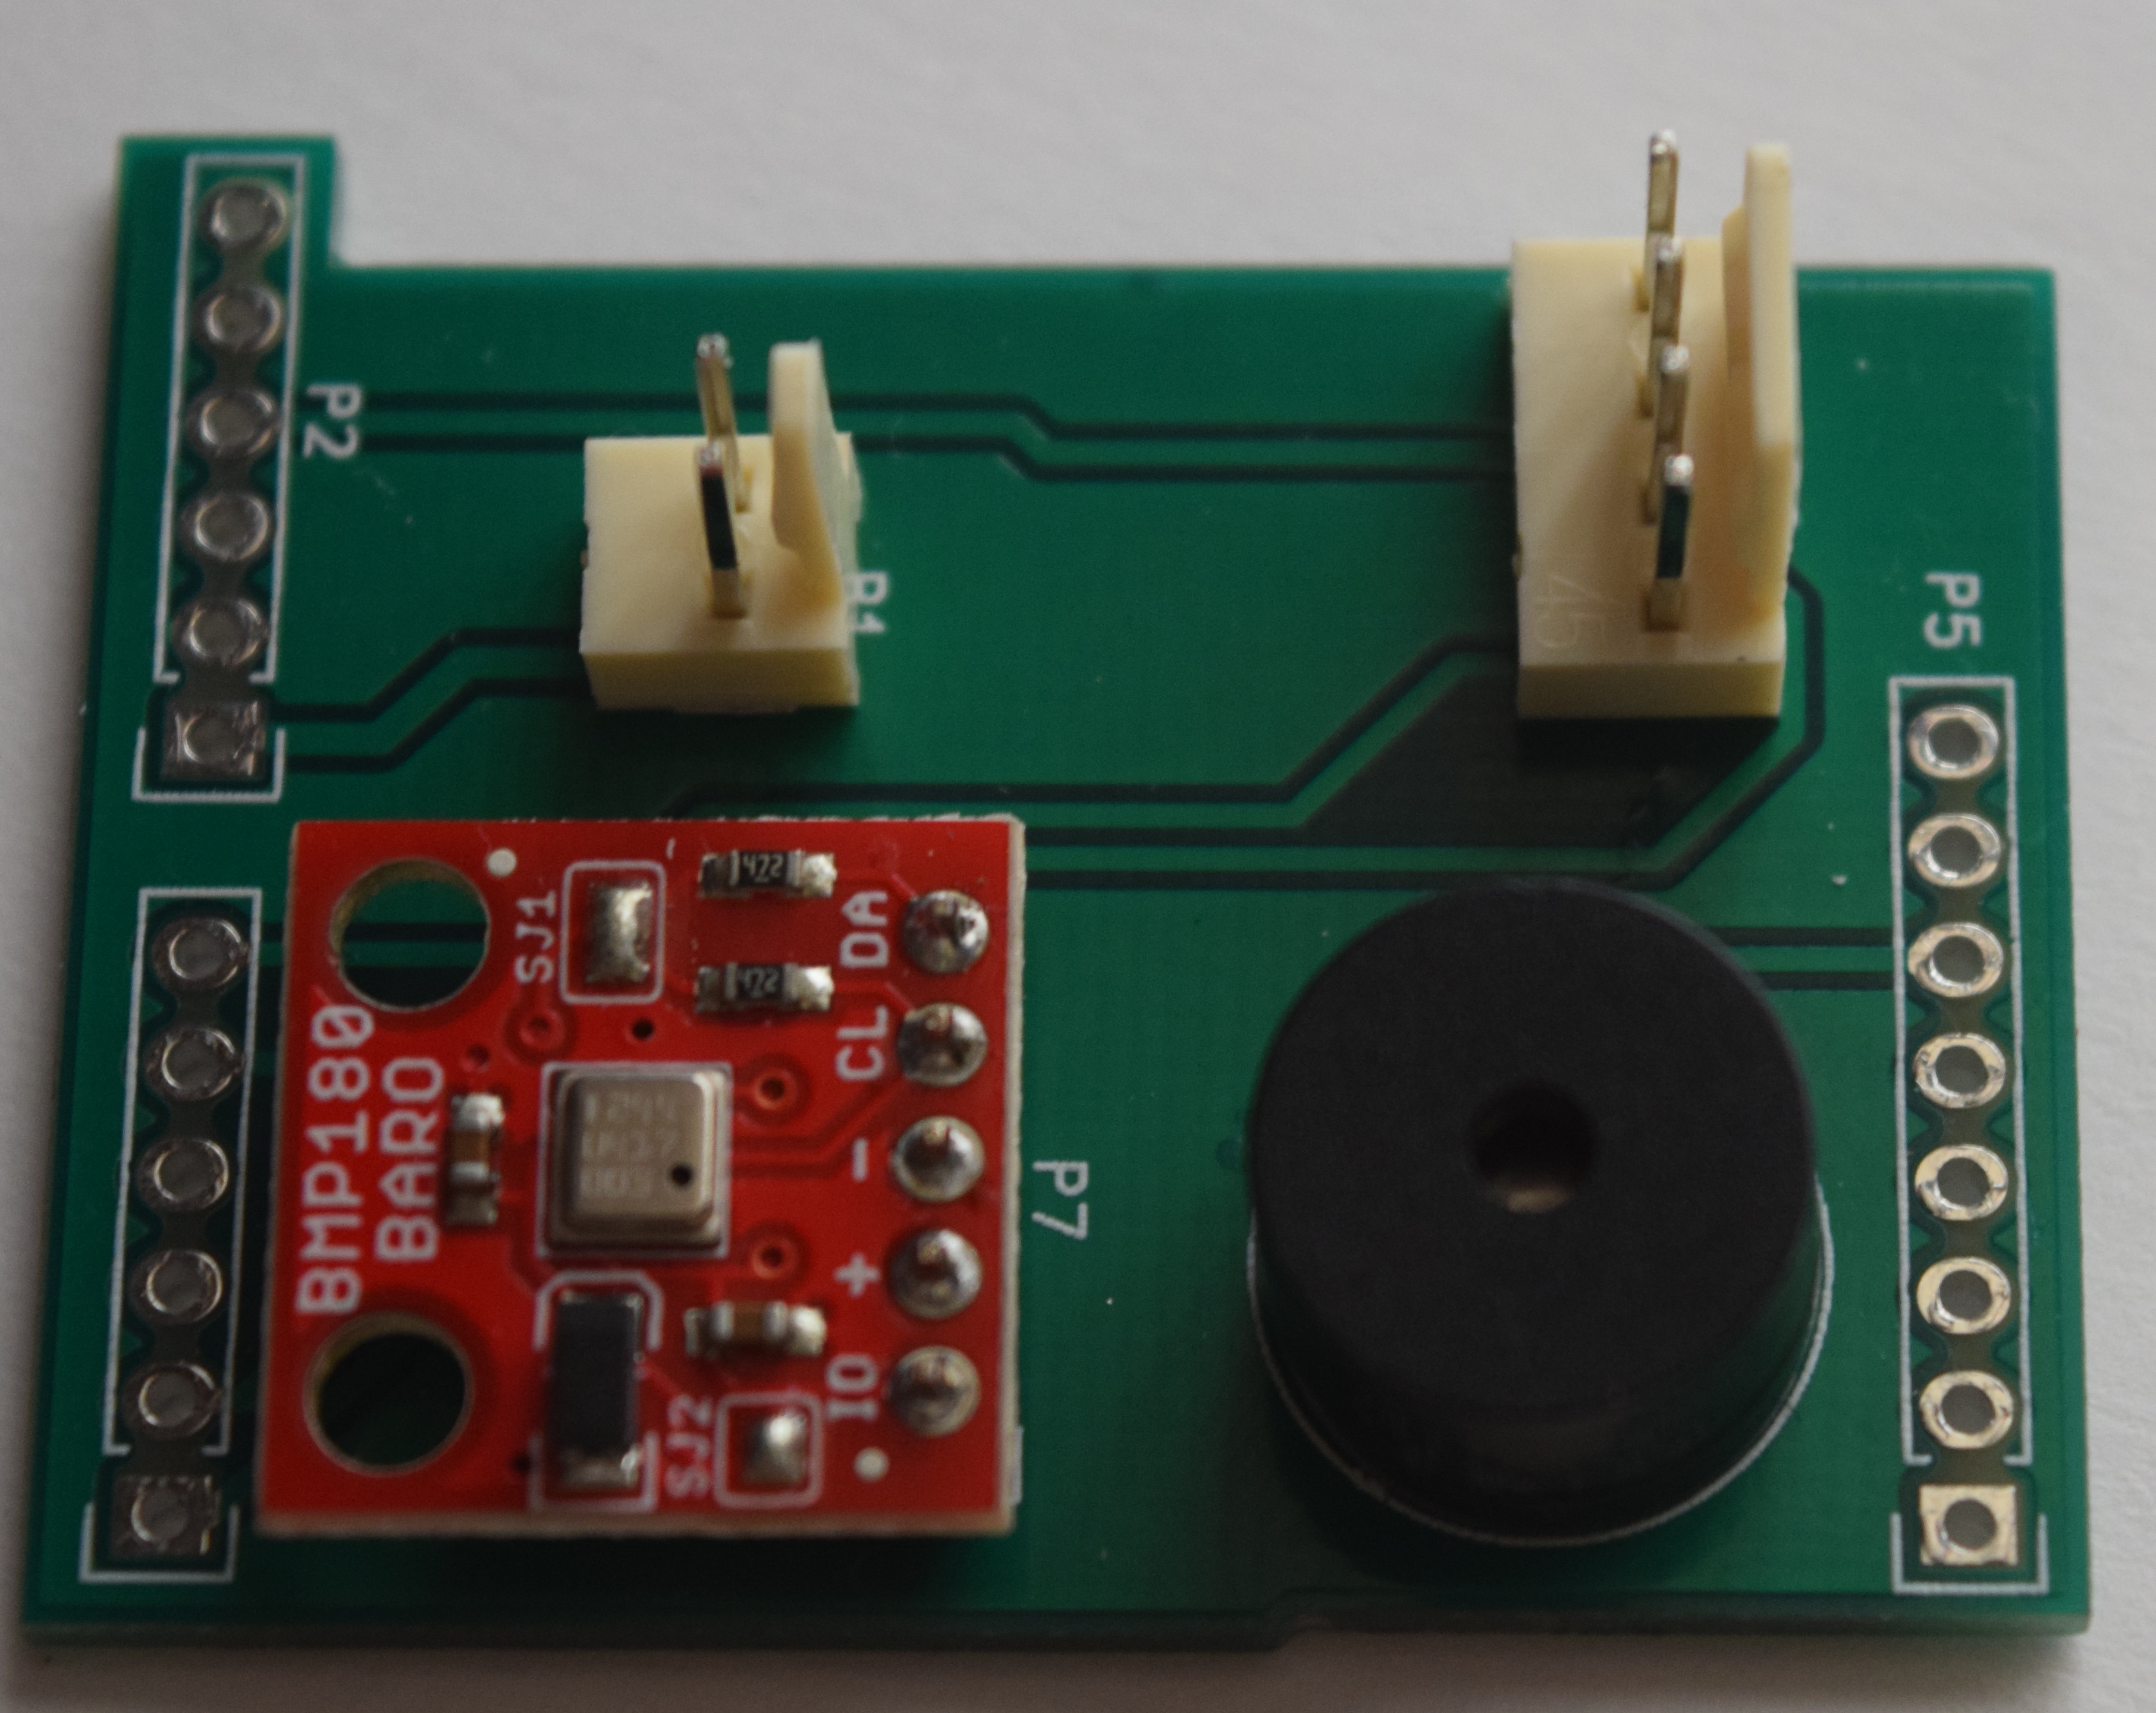
\includegraphics[width=\linewidth]{Figuras/figure_18_a.jpg}
    \center{(a)}
    \end{minipage}
    \centering
    \begin{minipage}{.45\textwidth}
    \centering
    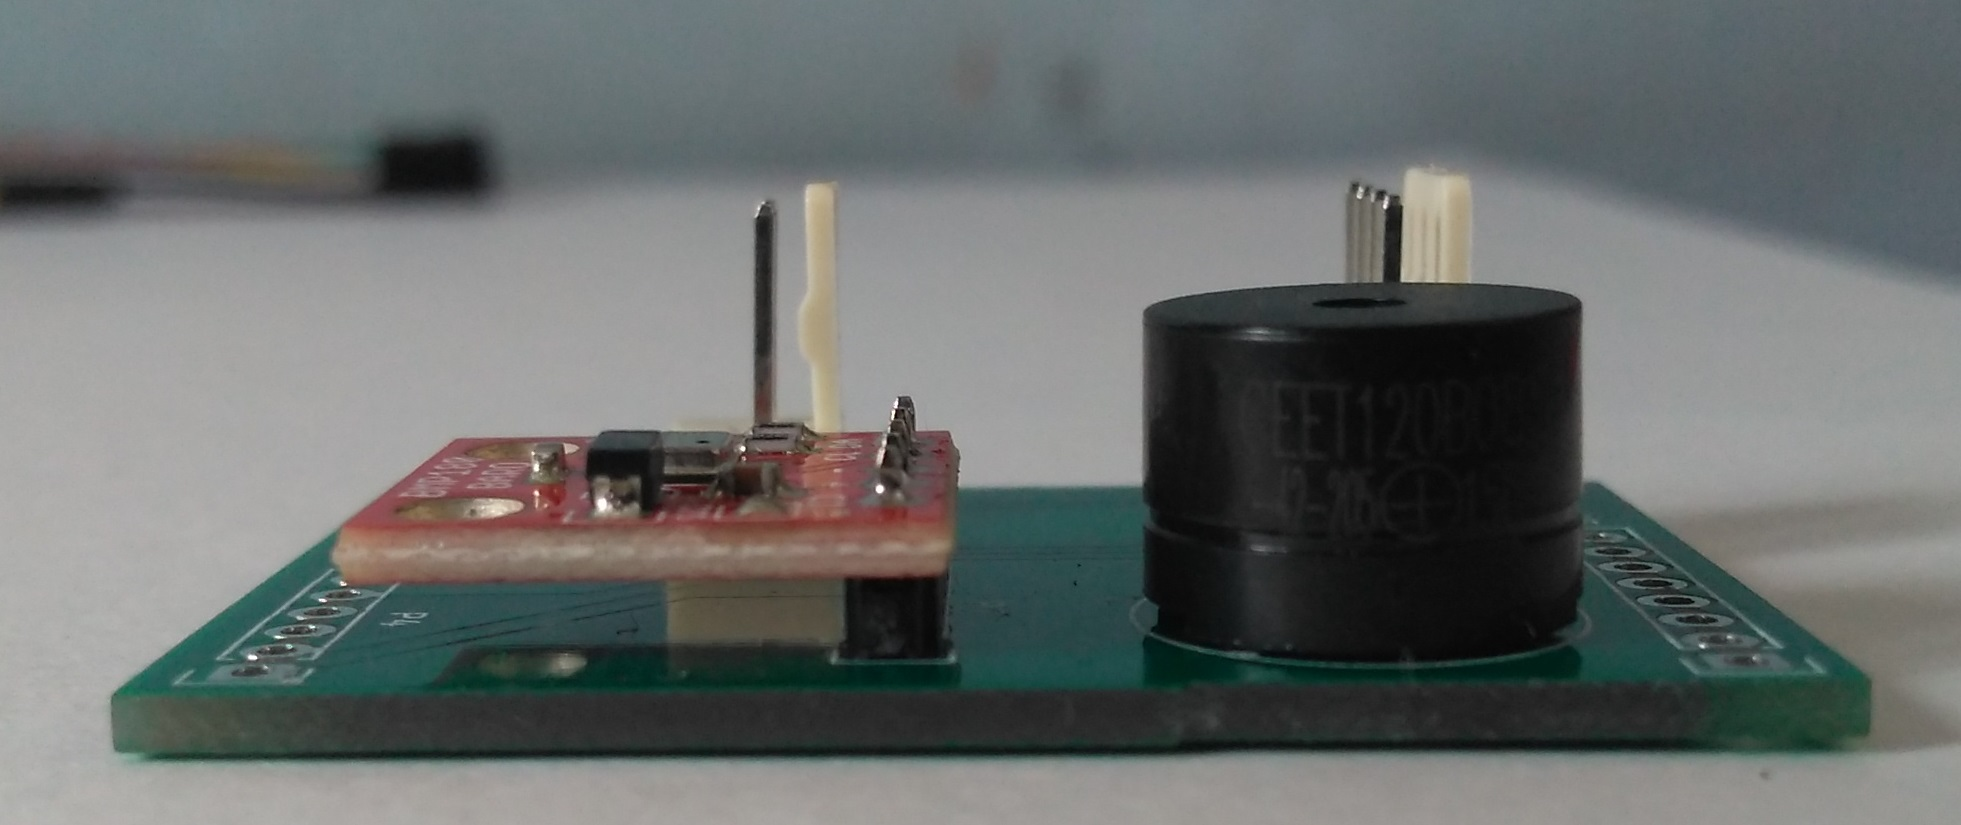
\includegraphics[width=\linewidth]{Figuras/figure_18_b.jpg}
    \center{(b)}
    \end{minipage}
    \centering
    \begin{minipage}{.45\textwidth}
    \centering
    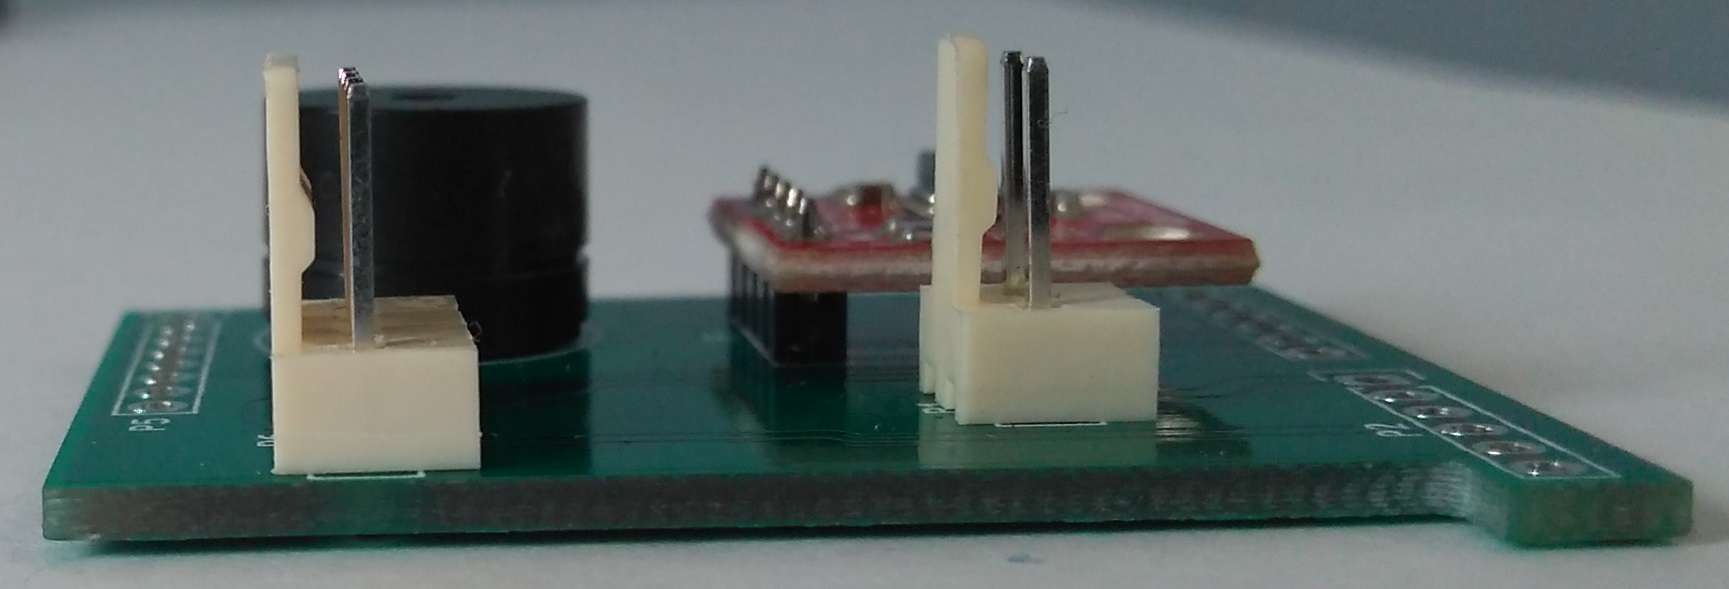
\includegraphics[width=\linewidth]{Figuras/figure_18_c.jpg}
    \center{(c)}
    \end{minipage}
    
    \caption{Assembled mini-board: (a) Top view, (b) Side view 1 and (c) Side view 2.}
    \label{fig:18}
\end{figure}

\begin{flushleft}
\textbf{(iv) Electrical connections}
\end{flushleft}

To communicate all the electronic components between each other it is necessary to connect them using cables. The use of a ribbon cable is highly recommended since it simplifies the identification of each cable through different colors and enables a better use of the space. In figure \ref{fig:19} is possible to see a ribbon cable with a Slim Housing of 1x1 in each side (black rectangle). Depending on the cable length it might be necessary to modify it for a better fit in the prototype structure (see section \ref{construccion}).

\begin{figure}[H]
    \centering
    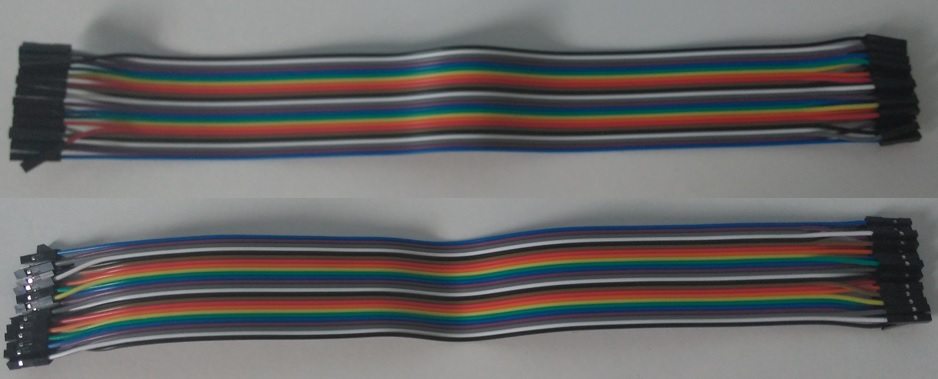
\includegraphics[scale=0.5]{Figuras/figure_19.jpg}
    \caption{Referential ribbon cable.}
    \label{fig:19}
\end{figure}

It is usefull to establish 3 cable sets for the electrical connections:

\begin{flushleft}
(iv.1) Battery connection - Switch - Armaduino and Data Logger
\end{flushleft}

To power the Armaduino a connection between the battery, the switch and the afformentioned board (through the male molex 2x1 soldered in the data logger) must be built. Figure \ref{fig:20} shows how should this connection look like. To see more details on the construction check section \ref{construccion}.

\begin{figure}[H]
    \centering
    \begin{minipage}{.45\textwidth}
    \centering
    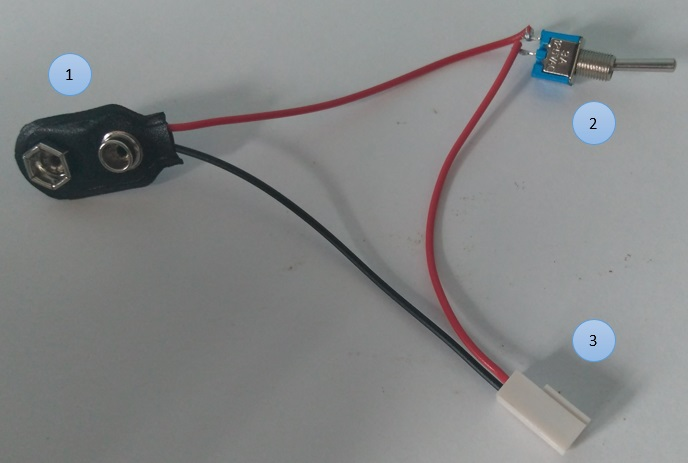
\includegraphics[width=\linewidth]{Figuras/figure_20_a.jpg}
    \center{(a)}
    \end{minipage}
    \centering
    \begin{minipage}{.45\textwidth}
    \centering
    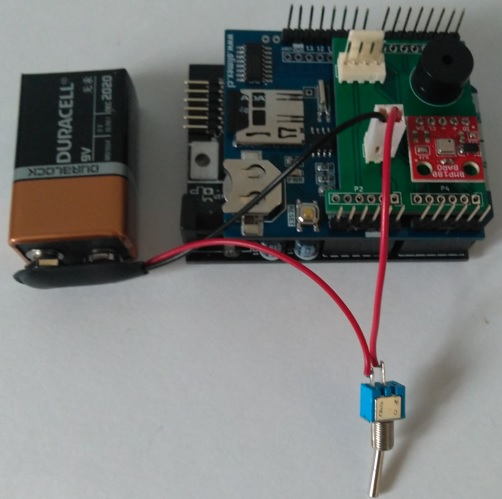
\includegraphics[width=\linewidth]{Figuras/figure_20_b.jpg}
    \center{(b)}
    \end{minipage}
        
    \caption{Battery connection - Switch - Armaduino and Data Logger: (a) Connection elements: (1) Battery conector, (2) Switch and (3) Female Molex 2x1. (b) Connection.}
    \label{fig:20}
\end{figure}

\begin{flushleft}
(iv.2) User interface connection - Armaduino and Data Logger
\end{flushleft}

This connection communicates the user interface with the Armaduino system to enable the screen feedback. It is composed by a total of 14 cables, shown in figure \ref{fig:21}, connecting the pin headers of the Interface PCB (figure \ref{fig:22}). The connectors used are referential and is recommended to minimize the amount of independent pieces, i.e. not using only 1x1 connectors. This improves the stability and reliability of the connections between each component.

\begin{figure}[H]
    \centering
    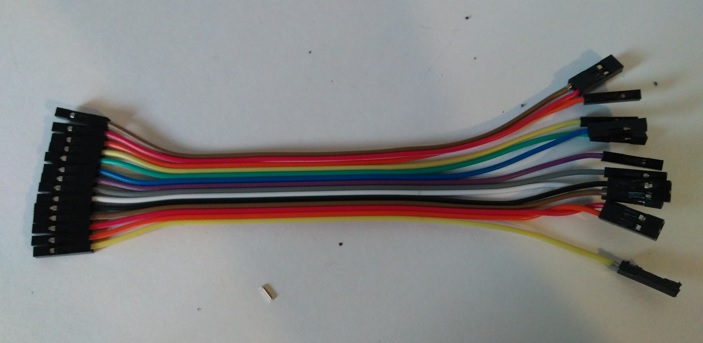
\includegraphics[scale=0.5]{Figuras/figure_21.jpg}
    \caption{Cable connection between the user interface and the Armaduino/Data Logger.}
    \label{fig:21}
\end{figure}

\begin{figure}[H]
    \centering
    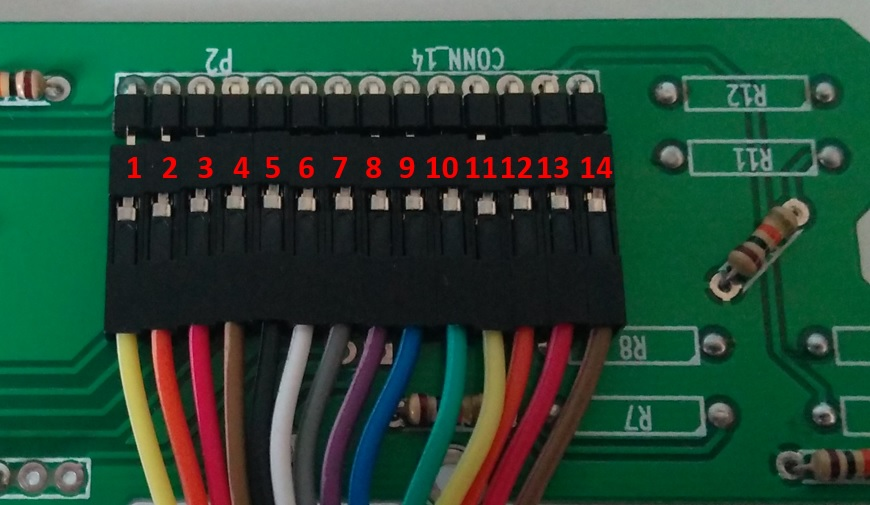
\includegraphics[scale=0.5]{Figuras/figure_22.jpg}
    \caption{Cable connection to the pin headers (footprint CONN\_14-P2) of the interface PCB, cables enumerated.}
    \label{fig:22}
\end{figure}

Next is the cable list showing where each labeled cable of Figure \ref{fig:22} is connected in the Armaduino:

\begin{itemize}
    \item Yellow Cable 1 $\rightarrow$ RST.
    \item Orange Cable 2 $\rightarrow$ TX.
    \item Red Cable 3 $\rightarrow$ RX.
    \item Brown Cable 4 $\rightarrow$ GND.
    \item Black Cable 5 $\rightarrow$ 5V.
    \item White Cable 6 $\rightarrow$ Digital Pin 9.
    \item Grey Cable 7 $\rightarrow$ Digital Pin 10.
    \item Purple Cable 8 $\rightarrow$ Digital Pin 6.
    \item Blue Cable 9 $\rightarrow$ Digital Pin 4.
    \item Green Cable 10 $\rightarrow$ Digital Pin 3.
    \item Yello Cable 11 $\rightarrow$ Digital Pin 2.
    \item Orange Cable 12 $\rightarrow$ Digital Pin 7.
    \item Red Cable 13 $\rightarrow$ Analog Pin 3.
    \item Brown Cable 14 $\rightarrow$ Analog Pin 2.
\end{itemize}

The cables position and installation is explained with more detail in section \ref{construccion}.

\begin{flushleft}
(iv.3) Sensor connection - Armaduino and Data Logger
\end{flushleft}

This bus connects the aerosol sensor with the Armaduino/Data Logger, transferring the amplified voltage measured by each LED for its registering in the microSD card of the datalogger. The connection is shown in figure \ref{fig:23}, where is possible to see how the cables are connected to the pin headers (P1 footprint in the sensor PCB), and to the male molex 4x1 of the data logger.

\begin{figure}[H]
    \centering
    \begin{minipage}{.45\textwidth}
    \centering
    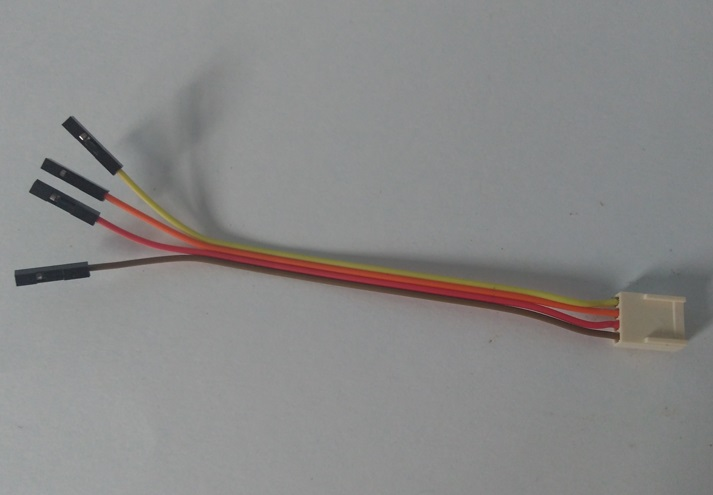
\includegraphics[width=\linewidth]{Figuras/figure_23_a.jpg}
    \center{(a)}
    \end{minipage}
    \centering
    \begin{minipage}{.45\textwidth}
    \centering
    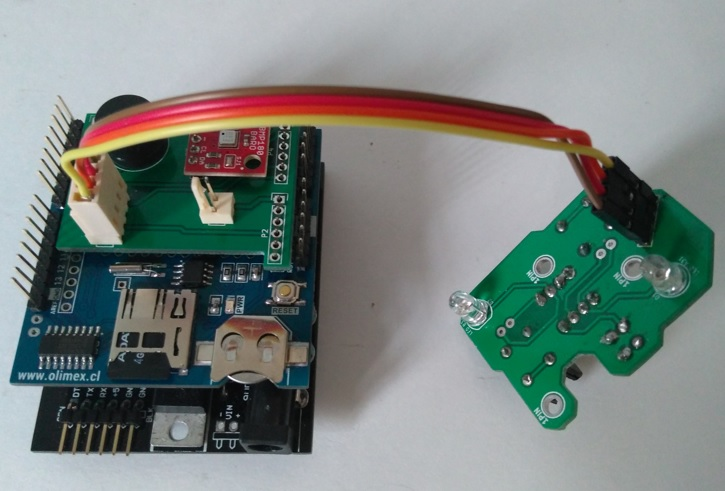
\includegraphics[width=\linewidth]{Figuras/figure_23_b.jpg}
    \center{(b)}
    \end{minipage}        
    \caption{Sensor connection - Armaduino/Data Logger: (a) Cables connection: Left side (Sensor) and right side (Data Logger), and (b) Sensor connection to the Armaduino/Data Logger.}
    \label{fig:23}
\end{figure}

For more building instructions and details check section \ref{construccion}.

\subsubsection{Structural components}

To optimize the layout of the electronic components (including thermal consideration of electronic), and to direct sunlight adequately towards the sensors, specific structural designs and components are used. The structural components are divided into External case (PVC pipe and covers) and Components printed in 3D.

 \begin{flushleft}
 \textbf{(i) External Case}
 \end{flushleft}

% La carcaza consiste en un tubo de PVC de 14.5 [cm] con dos tapas de PVC correspondientes para el diámetro del tubo. Estos elementos forman la carcaza externa del prototipo que se utiliza para proteger los componentes electrónicos y sostener la estructura formada por las piezas impresas en 3D. La figura \ref{fig:24} (a) muestra el tubo PVC y las dos tapas en su estado inicial y la figura \ref{fig:24} (b) muestra el tubo PVC y las tapas en su estado final luego de cortar el tubo PVC, cortar y pegar una de las tapas al tubo y cortar la otra tapa para ensamblarla con la estructura impresa en 3D.

The external case consists of a PVC pipe of 14.5 [cm] with two corresponding PVC covers for the diameter of the pipe. These elements form the external shell of the prototype that is used to protect the electronic components and to support the internal 3D printed structures. Figure \ref{fig:24}(a) shows the PVC tube and the two caps in their initial state and Figure \ref{fig:24}(b) shows the PVC tube and the caps in their final state after cutting the PVC tube (See section \ref{construccion}, \textit{Notes for the prototype construction}, for construction details of the external case.). 

 \begin{figure}[H]
     \centering
     \begin{minipage}{.45\textwidth}
     \centering
     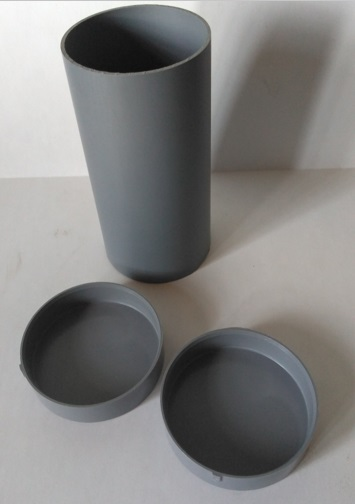
\includegraphics[width=\linewidth]{Figuras/figure_24_a.jpg}
     \center{(a)}
     \end{minipage}
     \centering
     \begin{minipage}{.45\textwidth}
     \centering
     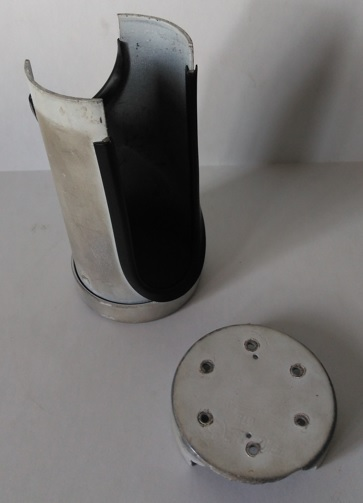
\includegraphics[width=\linewidth]{Figuras/figure_24_b.jpg}
     \center{(b)}
     \end{minipage}
        
     \caption{External case: (a) Materials (initial state) y (b) After adapting the components (final state). See section \ref{construccion}, \textit{Notes for the prototype construction}, for construction details of the external case.}
     \label{fig:24}
 \end{figure}


 \begin{flushleft}
 \textbf{(ii) 3D printed components} 
 \end{flushleft}

The 3D printed parts described below were printed on a Stratasys uPrint SE Plus printer, using ABS as a printing material. This printer reaches the required precision on the parts. Therefore, if another, less precise, 3D printer is used, the parts will have some dimensional variations that might affect the quality of the measurement. Also the difference in precision might generate differences with the parts shown in this document and in the dimensions of the external case.

Figure \ref{fig:25} shows the pieces printed in 3D. Figure \ref{fig:26} shows the assembly of the pieces 2, 3, 4, 6, 7, 8, 9 and 10 should look. Figure \ref{fig:27} shows how to assemble pieces 1 and 5 to the structure formed in Figure \ref{fig:26}. Figure \ref{fig:28} shows the final view of the internal structure, but without including the electronic components.

 \begin{figure}[H]
     \centering
     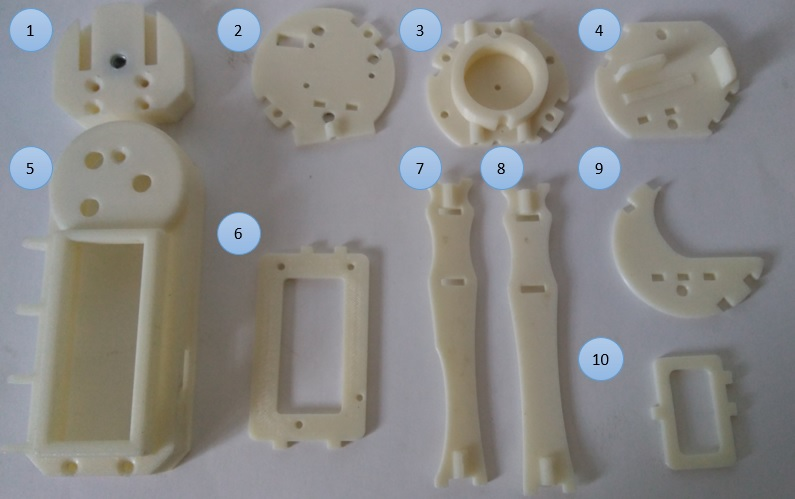
\includegraphics[scale=0.7]{Figuras/figure_25.jpg}
     \caption{3D-printed parts: (1) Tripod Adapter, (2) Sensor Support, (3) PVC Cap Support, (4) Battery Floor, (5) Control Panel Support, (6) Armaduino Support, (7) Lateral Support 01, (8) Lateral Support 02, (9) Armaduino Floor, (10) Battery Support.}
     \label{fig:25}
 \end{figure}

 \begin{figure}[H]
     \centering
     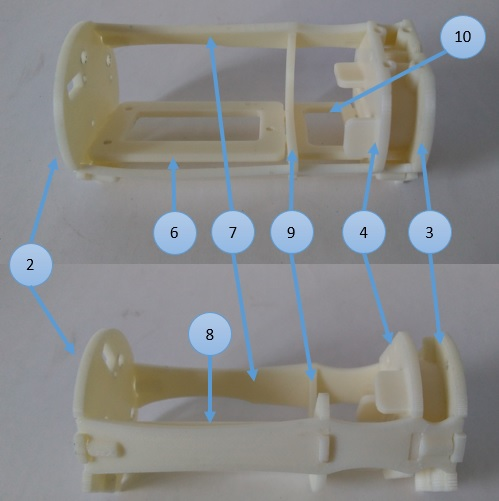
\includegraphics[scale=0.5]{Figuras/figure_26.jpg}
     \caption{Location in the structure of the 3D-printed parts: (1) Tripod Adapter, (2) Sensor Support, (3) PVC Cap Support, (4) Battery Floor, (5) Control Panel Support, (6) Armaduino Support, (7) Lateral Support 01, (8) Lateral Support 02, (9) Armaduino Floor, (10) Battery Support.}
     \label{fig:26}
 \end{figure}

 \begin{figure}[H]
     \centering
     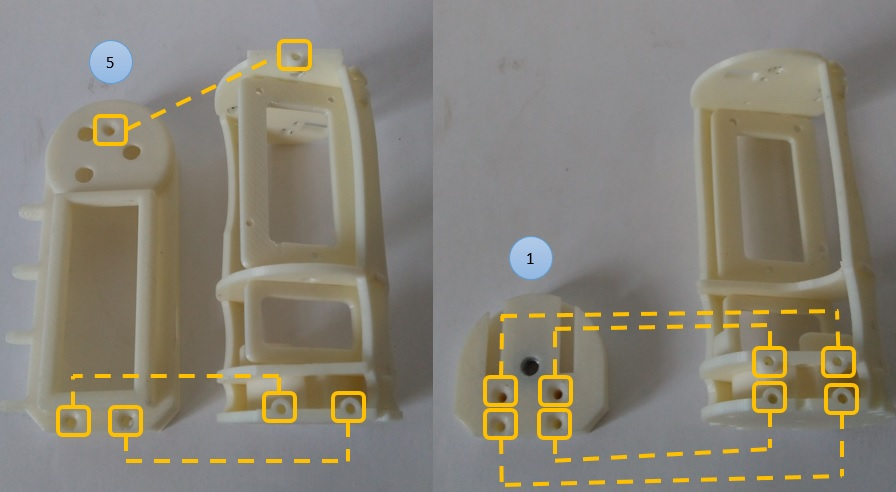
\includegraphics[scale=0.7]{Figuras/figure_27.jpg}
     \caption{Assembling the (1) Tripod Adapter to the (5) Control Panel Support.}
     \label{fig:27}
 \end{figure}

 \begin{figure}[H]
     \centering
     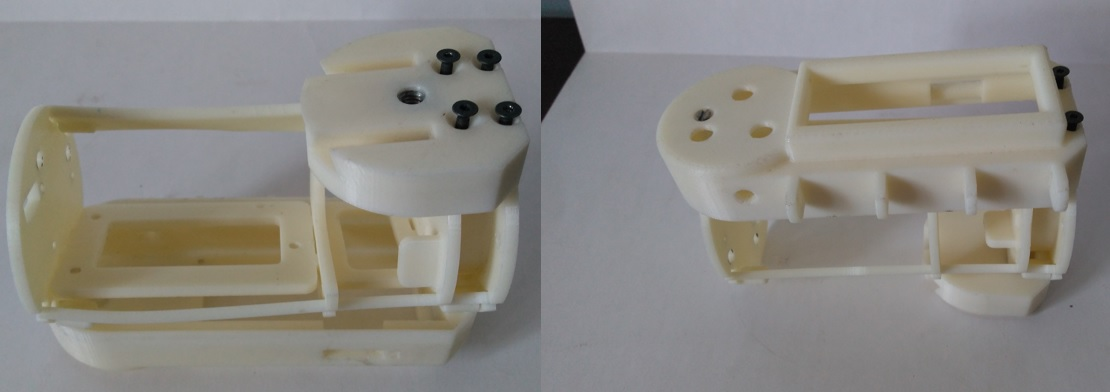
\includegraphics[scale=0.5]{Figuras/figure_28.jpg}
     \caption{Final view of 3D-printed parts, without the electronic components}
     \label{fig:28}
 \end{figure}



%****************************************FIN FELIPE********************************************************

%***************************************Comienzo Marcos*****************************************************

\newpage
\section{Notes for the prototype construction}\label{construccion}

\subsection{Electronic components}

\subsubsection{Steps to place the through-hole components on PCBs}

The steps to place the through-hole components on the PCBs are described in the following itemization: 

\begin{enumerate}
    \item Bend the components' pins depending on the spacing of the holes on the PCB board (Figure \ref{fig:29}).
    
\begin{figure}[H]
    \centering
    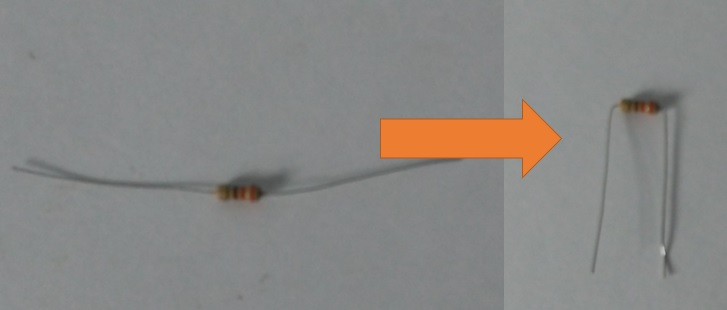
\includegraphics[scale=0.5]{Figuras/figure_29.jpg}
    \caption{How the wire pins have to be bent}
    \label{fig:29}
\end{figure}

    \item To facilitate soldering, when inserting the component it is recommended to bend the wire pins with the component close by to the PCB board (ideally touching the board) (figure \ref{fig:30}).
    
\begin{figure}[H]
    \centering
    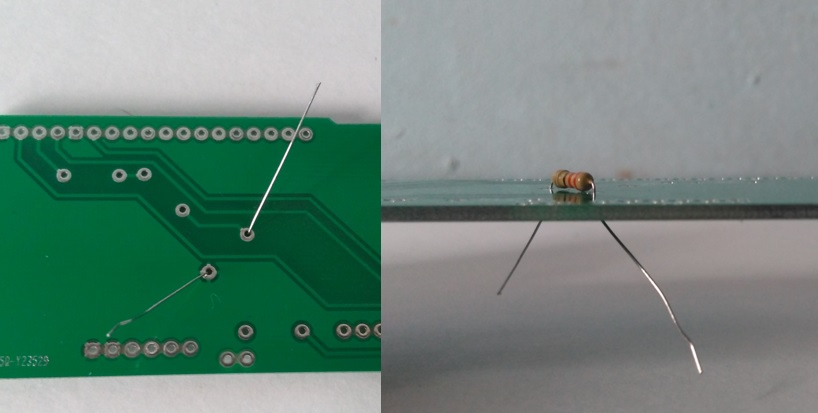
\includegraphics[scale=0.5]{Figuras/figure_30.jpg}
    \caption{Position of the component on the PCB board.}
    \label{fig:30}
\end{figure}

\end{enumerate}

\subsubsection{How to solder}

Once you have all the components for a system or subsystem you can go to the next step that is to solder the components. To do this, follow these steps:

\begin{enumerate}
    \item Heat the pin and the metallic part of the hole with the soldering iron.
    \item Add soldering by touching the pin wire and the metallic part of the hole with the soldering wire.
    \item Remove the soldering wire.
    \item Remove the soldering iron. Be sure the soldering is in contact with both the pin wire of the component and the metallic part of the hole. 
\end{enumerate}

Figure \ref{fig:31} graphically shows the steps listed above. Figure \ref{fig:32} shows examples of a correct and incorrect soldering. If the shape of the soldering gets an incorrect shape, then clean the soldering iron tip (when it is off and cold) and then reheat it, melting the soldering until it takes the correct shape.

\begin{figure}[H]
    \centering
    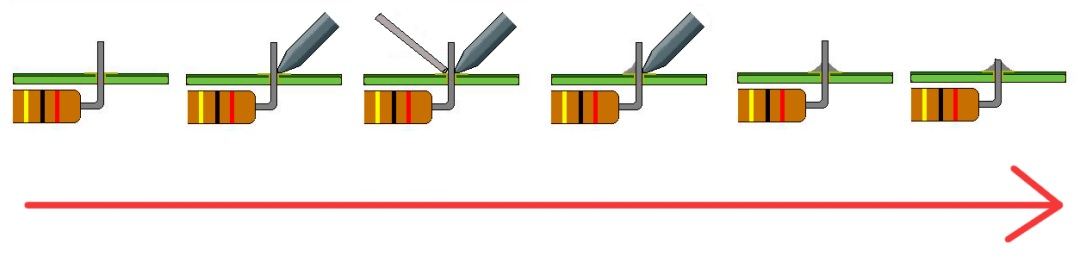
\includegraphics[scale=0.5]{Figuras/figure_31.jpg}
    \caption{Steps for soldering \cite{Armaduino}.}
    \label{fig:31}
\end{figure}

\begin{figure}[H]
    \centering
    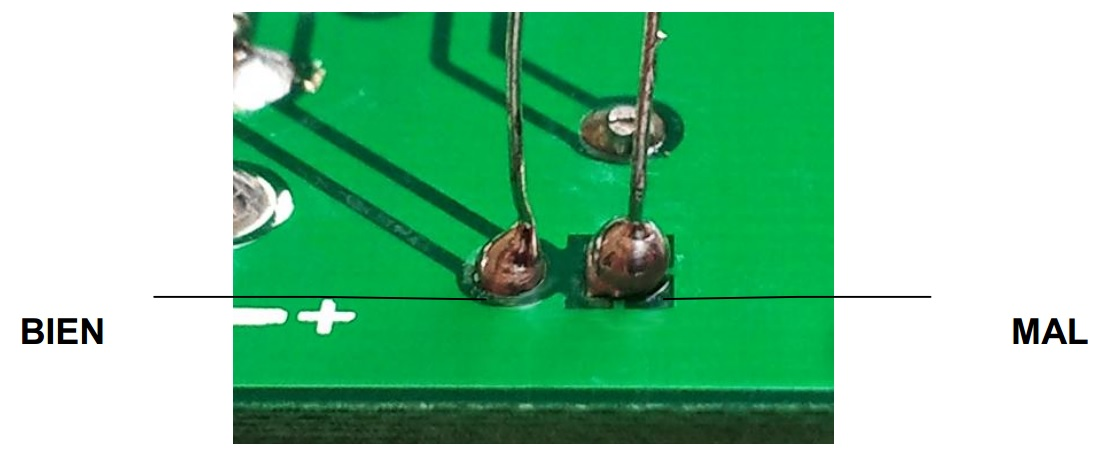
\includegraphics[scale=0.5]{Figuras/figure_32.jpg}
    \caption{Correct soldering (left: correct shape of soldering) e incorrect (right: incorrect shape of soldering) \cite{Armaduino}.}
    \label{fig:32}
\end{figure}

If the person doing the soldering has not previously soldered, it is recommended to let the person practice on a practice board in order to avoid problems during soldering of the actual system. Extra attention and practice should be paid if the used soldering iron does not allow temperature regulation.

\subsubsection{Connections}

In section \ref{componentes_electronicos}, (iv) the connection procedure among components was described. The used cables are connected through two types of components: (1) Housing Slim and (2) Molex, with their respective terminals which are shown in figure \ref{fig:33}.

\begin{figure}[H]
    \centering
    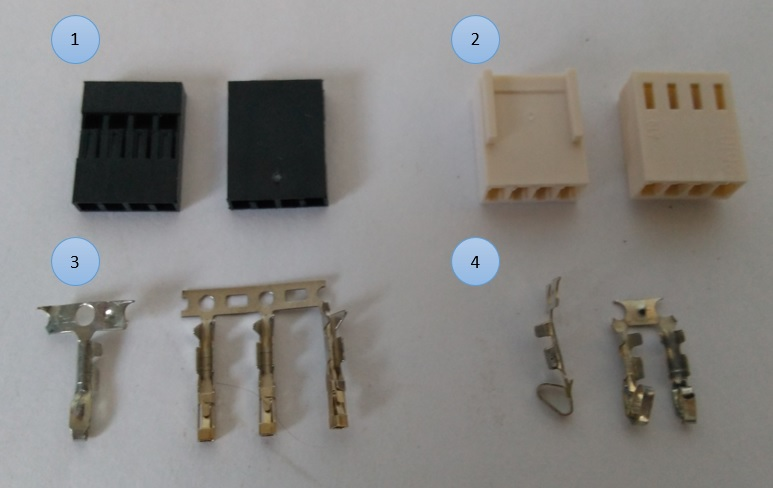
\includegraphics[scale=0.45]{Figuras/figure_33.jpg}
    \caption{Conectors: (1) Housing Slim; (2) Molex female, and Terminals: (3) Housing Slim; and (4) Molex.}
    \label{fig:33}
\end{figure}


The steps for generating the cable connection to the terminal and the subsequent assembly with the connector are described below and are shown in the figure \ref{fig:34}:

\begin{itemize}
	\item \underline{Step 1}: Give to the cable the desired length.
	\item \underline{Step 2}: Peel the end of the cable.
 	\item \underline{Step 3}: Put the stripped cable end on the terminal so that the plastic is between the tabs as indicated in the yellow circle of figure \ref{fig:34} (3). 
	\item \underline{Step 4}: Weld the bare part of the cable to the terminal so that they are joined together. Care should be taken to put the soldering iron on the terminal for a too long time since it may cause the plastic to melt impeding contact.
	\item \underline{Step 5}: Fold the eyelashes indicated in the yellow circle in figure \ref{fig:34} (4) so that they embrace the cable as shown in figure \ref{fig:34} (5).
	\item \underline{Step 6}: Locate the connector and the terminal as shown in figure \ ref {fig:34} (6).
	\item \underline{Step 7}: Insert the cable in the end until you hear a "click". The terminal must be completely inside the connector.
\end{itemize}

\begin{figure}[H]
    \centering
    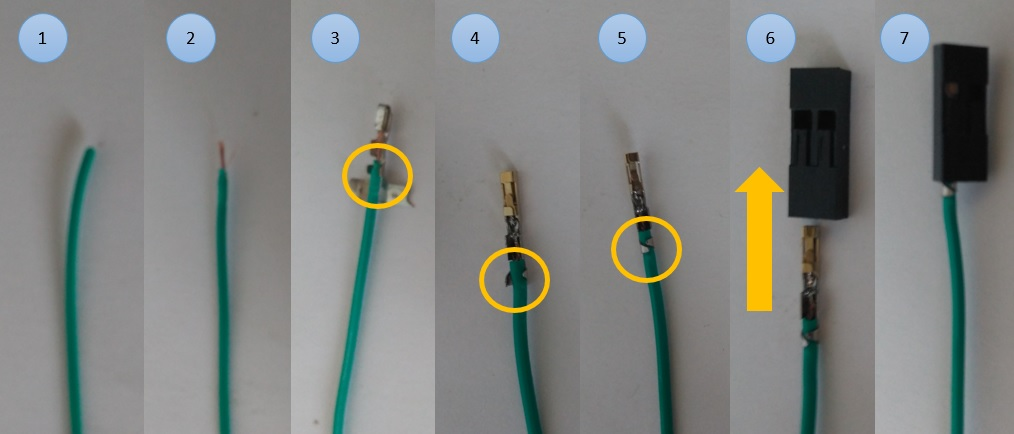
\includegraphics[scale=0.5]{Figuras/figure_34.jpg}
    \caption{Steps to do a connector with Housing Slim.}
    \label{fig:34}
\end{figure}

The procedure is equivalent for a molex terminal. The way of inserting the terminal into the molex connector is shown in figure \ref{fig:35}.

\begin{figure}[H]
    \centering
    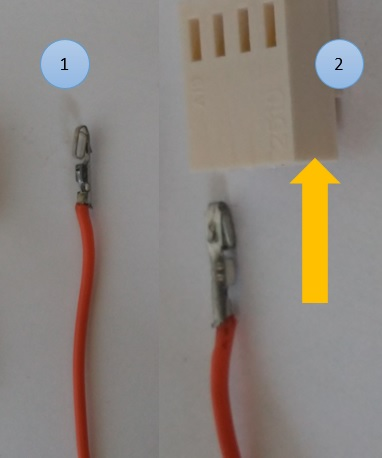
\includegraphics[scale=0.6]{Figuras/figure_35.jpg}
    \caption{Steps to insert the molex terminal in the molex connector.}
    \label{fig:35}
\end{figure}

\subsection{External case}

This section specifies the dimensions of the cuts that need to be made in both the PVC tube and the lids in order to go from what is shown in the figure \ ref {fig: 24} (a) to what is shown in the figure \ref{fig:24}(b).

The steps for cutting the PVC tube and the caps are described below and are shown from the figure \ref{fig:36} to the figure \ref{fig:40} (the images are distorted due to the camera angle):

\begin{itemize}
\item \underline{Paso 1}: Glue the PVC tube to one of the caps and at the free end mark the PVC edges that have a distance of 5.5 [cm] as shown in the figure \ref{fig:36}.
    
    \begin{figure}[H]
        \centering
        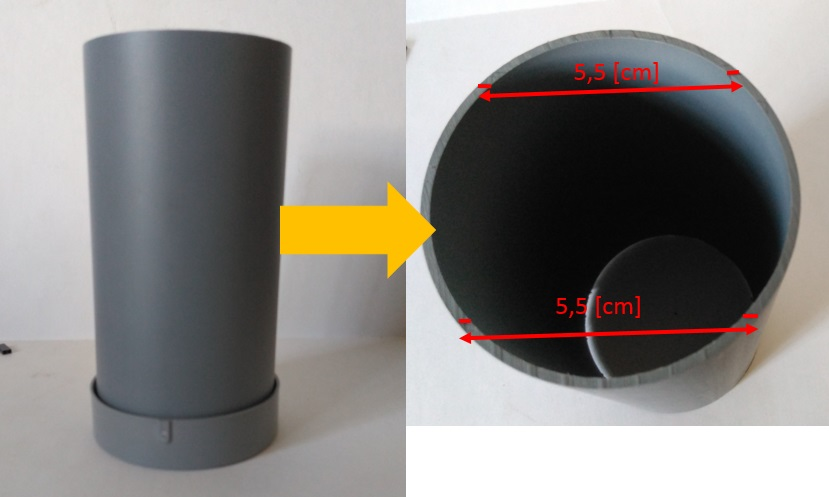
\includegraphics[scale=0.6]{Figuras/figure_36.jpg}
        \caption{Step 1. External case (Tube and caps).}
        \label{fig:36}    
    \end{figure}
    
\item \underline{Paso 2}: From each of the marked edges, which are described the previous step and shown figure \ref{fig:36} right): (edge 1) draw 2 parallel vertical lines of 11 [cm] each. At the end of the lines draw a semi-circle of 2.75 [cm] in radius (notice that the radius is the half of the 5.5 [cm] marked in the previous step) (edge 2) draw 2 parallel vertical lines of 2 [cm] each. At the end of the lines draw a semi-circle of 2.75 [cm] in radius. This step is graphically summarized in figure \ref{fig:37}.

    \begin{figure}[H]
        \centering
        \includegraphics[scale=0.6]{Figuras/figure_37.jpg}
        \caption{Step 2. Marks for cuts to the external case.}
        \label{fig:37}    
    \end{figure}
    
Due to the shape of the pipe, it can be difficult to mark the described dimensions, so that, it is recommended to mark the nearest dimensions, cut and adjust later (filing the edges until reach the desired dimensions).

\item \underline{Paso 3}: Cut following the marked lines of the previous step, then paint and put the rubber over the edges as shown in figure \ref{fig:38}.

    \begin{figure}[H]
        \centering
        \includegraphics[scale=0.6]{Figuras/figure_38.jpg}
        \caption{Step 3. Cuts to the external case.}
        \label{fig:38}    
    \end{figure}
    
\item \underline{Paso 4}: On the other cap the edges must be cut off. To do so, mark the edges that are separed by 4 [cm] as shown in figure \ref{fig:39} (left). Once the edges have been marked, mark the edge of the cap with the dimensions shown in the figure \ref{fig:39} (right). Do this on both sides and then cut.

    \begin{figure}[H]
        \centering
        \includegraphics[scale=0.5]{Figuras/figure_39.jpg}
        \caption{Step 4. Cuts in top cap. C}
        \label{fig:39}    
    \end{figure}
    
\item \underline{Paso 5}: To assemble the external cap with the 3D part, place the center of the top cap and line it with the center hole of the 3D part that should be assembled with the top cap (the one with tiny holes for capturing sun light) as shown in figure \ref{fig:40} (Left, red circle)). Then mark all the holes in the top PVC cap, paying extra attention to the small holes in the figure \ref{fig:40} (Left, green circle) since these holes will allow the light to arrive to the LED sensors. It is recommended to use a small drill (ex. Dremel) with the same diameter of the tiny holes and later to increase the diameter of the orifices on the top PVC cap.

    \begin{figure}[H]
        \centering
        \includegraphics[scale=0.6]{Figuras/figure_40.jpg}
        \caption{Paso 5. Assembling top PVC cap with the corresponding 3D part.}
        \label{fig:40}    
    \end{figure}
    
\end{itemize}


\subsection{Assembling}

%OJO CREO QUE NO SE OCUPAN PERNOS SINO QUE TORNILLOS (ESTO SEGUN LAS FOTOS) LOS PERNOS NECESITAN LLAVE Y NO ATORNILLADORES
%
%NOTAR QUE EN MUCHA SPARTE DICE ARMADUINO EN LUGAR DE ARDUINO YO CAMBIE ESTO PERO CREO ESTA ASI EN EL CAPITULO 2 TAMBIEN. 
%
%OJO QUE HAY QUE SER CONSISTENTE EN LOS NOMBRES DE LAS PIEZAS A CASI TODOS LOS SOPORTES LOS TRADUJE COMO SUPPORT (EJ. ARDUINO SUPPORT POR SOPORTE DE ARDUINO)

With the electronic and structural components ready, the components must be assembled. For assembling the electronic components with the 3D parts are used screw of different diameter and type, which are detailed in table \ref{tab:3}.

\begin{table}[H]
\centering
\caption{Type and location of assembling screws.}
\label{tab:3}
\begin{tabular}{|l|r|l|}
\hline
\textbf{Screw} & \multicolumn{1}{l|}{\textbf{Quantity}} & \textbf{Location}  \\ \hline
Conic screw 2mmx18mm parker & 4 & Tripod adapter   \\ \hline
Screw 2mmx22mm  & 1   & Control panel support \\ \hline
Conic screw 2mmx18mm parker & 2 & Control panel support \\ \hline
Screw 3mmx10mm & 6 & PVC cap \\ \hline
Screw 2mmx10mm & 3 & User interface   \\ \hline
Screw 3mmx5mm & 2  & Sensor   \\ \hline
Screw 3mmx11mm & 1 & Lateral support 01  \\ \hline
Screw 3mmx11mm & 1 & Lateral support 02  \\ \hline
\end{tabular}
\end{table}

The assembly procedure follows the following steps:

\begin{itemize}
\item \underline{Step 1}: Assemble PVC Cap with PVC Cap support except for the holes shown in figure \ref{fig:41}.

    \begin{figure}[H]
        \centering
        \includegraphics[scale=0.6]{Figuras/figure_41.jpg}
        \caption{Assembling procedure. Step 1.}
        \label{fig:41}    
    \end{figure}
    
    \item \underline{Step 2}: Assembling the Arduino with its support (Arduino Support in figure \ref{fig:25}). See figure \ref{fig:42}).
    
    \begin{figure}[H]
        \centering
        \includegraphics[scale=0.5]{Figuras/figure_42.jpg}
        \caption{Assembling procedure. Step 2.}
        \label{fig:42}    
    \end{figure}
    
\item \underline{Step 3}: Connect to the Arduino the Data Logger, the sensor and the user interface buses (see figure \ref{fig:43}).

    \begin{figure}[H]
        \centering
        \includegraphics[scale=0.5]{Figuras/figure_43.jpg}
        \caption{Assembling procedure. Step 3.}
        \label{fig:43}    
    \end{figure}
    
    \item \underline{Step 4}: Assemble the sensor to its mounting (Sensor Support in figure \ref{fig:25}).). See figure \ref{fig:44}).
    
    \begin{figure}[H]
        \centering
        \includegraphics[scale=0.5]{Figuras/figure_44.jpg}
        \caption{Assembly procedure. Step 4.}
        \label{fig:44}    
    \end{figure}
    
    \item \underline{Step 5}:  Assemble the user interface with the Control Panel Support (figure \ref{fig:25}) as shown in figure \ref{fig:45}.
    
    \begin{figure}[H]
        \centering
        \includegraphics[scale=0.5]{Figuras/figure_45.jpg}
        \caption{Assembly procedure. Step 5.}
        \label{fig:45}    
    \end{figure}
    
\item \underline{Step 6}: Install the switch connection in the Control Panel Support (figure \ref{fig:25}) as shown in figure \ref{fig:46}.

    \begin{figure}[H]
        \centering
        \includegraphics[scale=0.5]{Figuras/figure_46.jpg}
        \caption{Assembly procedure. Step 6.}
        \label{fig:46}    
    \end{figure}
    
\item \underline{Step 7}: Connect the Arduino with the user interface. Connect the Switch connection to the Arduino (see figure \ref{fig:47}.).

    \begin{figure}[H]
        \centering
        \includegraphics[scale=0.5]{Figuras/figure_47.jpg}
        \caption{Assembly procedure. Step 7.}
        \label{fig:47}    
    \end{figure}
    
\item \underline{Step 8}: Connect the sensor to the Arduino. Assemble the Arduino Support to the Arduino Floor and Sensor Support (see figures \ref{fig:25} and \ref{fig:48})

    \begin{figure}[H]
        \centering
        \includegraphics[scale=0.5]{Figuras/figure_48.jpg}
        \caption{Assembly procedure. Step 8: (1) Sensor Support and (2) Arduino Floor.}
        \label{fig:48}    
    \end{figure}
    
    \item \underline{Step 9}: Assemble the Battery Support with Arduino Floor (see figure \ref{fig:49}). 
    
    \begin{figure}[H]
        \centering
        \includegraphics[scale=0.5]{Figuras/figure_49.jpg}
        \caption{Assembly procedure. Step 9: (1) Arduino Floor and (2) Battery Support.}
        \label{fig:49}    
    \end{figure}
    
    \item \underline{Step 10}: Assemble the battery Support with the Battery Floor (see figure \ref{fig:50}). 
    
    \begin{figure}[H]
        \centering
        \includegraphics[scale=0.5]{Figuras/figure_50.jpg}
        \caption{Assembly procedure. Step 10: (1) Battery Support y (2) Battery Floor.}
        \label{fig:50}    
    \end{figure}
    
\item \underline{Step 11}: Put the Side Supports in the slots with the Sensor Support, Arduino Floor and Battery Floor. Assemble with Sensor Support (see figures \ref{fig:51} and \ref{fig:51_2}).

    \begin{figure}[H]
        \centering
        \includegraphics[scale=0.5]{Figuras/figure_51.jpg}
        \caption{Assembly procedure. Step 11.1: (1) Side Support 01 and (2) Side Support 02.}
        \label{fig:51}    
    \end{figure}
    
    \begin{figure}[H]
        \centering
        \includegraphics[scale=0.5]{Figuras/figure_51_2.jpg}
        \caption{Assembly procedure. Step 11.2: Assembly with Sensor Support.}
        \label{fig:51_2}    
    \end{figure}
    
\item \underline{Step 12}: Put into the slots with the PVC Cap Support and screw to assemble (see figure \ref{fig:52}).

    \begin{figure}[H]
        \centering
        \includegraphics[scale=0.5]{Figuras/figure_52.jpg}
        \caption{Assembly procedure. Step 12.}
        \label{fig:52}    
    \end{figure}
    
    \item \underline{Step 13}: Screw to assemble the Control Panel Support to the structure (see figure \ref{fig:53}).
    
    \begin{figure}[H]
        \centering
        \includegraphics[scale=0.5]{Figuras/figure_53.jpg}
        \caption{Assembly procedure. Step 13.}
        \label{fig:53}    
    \end{figure}
    
    \item \underline{Step 14}: Assemble the Tripod Adaptor to the structure (see figure \ref{fig:54}).
    
    \begin{figure}[H]
        \centering
        \includegraphics[scale=0.5]{Figuras/figure_54.jpg}
        \caption{Assembly procedure. Step 14.}
        \label{fig:54}    
    \end{figure}
    
    \item \underline{Step 15}: Put the battery in the Battery Support and connect to the system (see figure \ref{fig:55}).
    
    \begin{figure}[H]
        \centering
        \includegraphics[scale=0.5]{Figuras/figure_55.jpg}
        \caption{Assembly procedure. Step 15.}
        \label{fig:55}    
    \end{figure}
    
    \item \underline{Paso 16}: Turn on the system (The Arduino must be previously programmed and configured). The screen should display a message as the one shown in figure \ref{fig:56}.
    
    \begin{figure}[H]
        \centering
        \includegraphics[scale=0.5]{Figuras/figure_56.jpg}
        \caption{Assembly procedure. Step 16.}
        \label{fig:56}    
    \end{figure}
    
\end{itemize}




%%%%%%%%%%%%%%%%%%%%%%%Fin traduccion Marcos%%%%%%%%%%%%%%%%%%%%%%

\newpage

\section{Data Extraction}

After performing at least one measurement, a .csv file is generated and stored on the microSD card. This file can be opened with a spreadsheet software. Within the file is the information recorded by the instrument in 12 columns: (1) Year, (2) Month, (3) Day, (4) Hour, (5) Minutes, (6) Seconds, (7) Sensor at 564 [Nm] (yellow LED), (8) Sensor at 408 [nm] (Blue LED), (9) Temperature, (10) Pressure, (11) Altitude and (12) ID.

The maximum voltages (and data from all columns for the corresponding row) must be extracted for each sensor at a defined time interval.

\section{Calibration}

\subsection{Langley-Plot}

To use the equation \ref{eq:001} it is necessary to obtain the value of the calibration constant $ V_0 $. To obtain this value two complementary methods of calibration are used.

The first method is to use the Langley Plot procedure with the instrument. The calibration constant is obtained by mapping the logarithm of the measured voltage under different air mass conditions (make measurements for different zenith angles), and then comparing with the equation \ref{eq:6}, this equation assumes the approximation of \textit{equivalent wavelength} described for the equation \ref{eq:001}.

\begin{equation}
    \ln V = \ln\left(V_0 \left(\frac{R_0}{R} \right)^2\right) - \left(\alpha_R \frac{P}{P_0} + \alpha_a\right)m_{air}
    \label{eq:6}
\end{equation}

To use this procedure some conditions must be met:


\begin{itemize}
    \item The sky must be completely clear, without clouds.
    \item Measurements should be made above 3000 meters of altitude from sea level.
    \item It is recommended that the zenith angles of the measurements to be less than 70$^{\circ}$.
\end{itemize}

When the number of measurements is sufficient, the voltage logarithm is plotted as function of the air mass, which is related to the zenith angles. A linear model is fitted to the data, $y=mx+n$, where $ m $ is the slope of the line and $n$ is the position coefficient. Then the value of the calibration constant is given by,

\begin{equation}
    n=ln(V_0(\frac{R_0}{R})^2)
    \label{eq:7}
\end{equation}

The Langley Plot calibration procedure of one of the sun photometer prototype is shown in Figure \ref{fig:57}. The Langley Plot procedure is performed at an altitude over most of the mankind-produced aerosols, however this procedure does not account for the gases effect on the measurements. Commercial instruments solve this problem by using narrow wavelength band filters in front the detectors. We do not use these filters in our instrument. Currently one of the most important factors in the high cost of the sun photometers are these filters. Therefore, the systematic error, made by using a broad-bandwidth sensor, must be corrected. It is done by using side-by-side measurements with a standard patron instrument.

\begin{figure}[H]
    \centering
    \includegraphics[scale=0.7]{Figuras/figure_57.png}
    \caption{Example of a Langley Plot obtained with one of the sun photometer prototypes. It can be seen that the results match the expected results for a monochromatic Langley Plot.}
    \label{fig:57}    
\end{figure}

\subsection{Correction with a patron instrument}

To correct the calibration constant obtained with the Lagnley Plot, measurements must be made side by side with a standard patron instrument.  Thus, AOT measurements are simultaneously taken with both instruments. 

To improve the calibration data, it is recommended to over measure (or sample) with the prototype respect to the patron instrument. Subsequently, the data of the prototype is filtered (decimated) leaving only the maximum value obtained for a time range equal to $\pm 3$ minutes with respect to the measurement time of the patron instrument. This is done to reduce the influence of the operator on the quality of the data.

If the prototype and the patron instrument do not measure the AOT at the same wavelengths, the measurements made by the patron instrument must be adjusted.  For this reason, the exponential formula of {\AA}ngstr\"{o}m (Eq. \ref{eq:8}) is used to do so. Thus, the AOT values of the patron instrument are interpolated to the prototype wavelengths.

\begin{equation}
    \frac{\tau_{\lambda}}{\tau_{\lambda_0}} = \left(\frac{\lambda}{\lambda_0}\right)^{-\alpha}, 
    \label{eq:8}
\end{equation}


where $\tau_{\lambda}$ is the optical thickness at the wavelength $\lambda$, $\tau_{\lambda_0}$ is the optical thickness at the reference wavelength and $\alpha$ is the {\AA}ngstr\"{o}m coefficient. Then it is possible to calculate the AOT at an equivalent wavelength with the coefficient {\AA}ngstr\"{o}m coefficient and the measurements of the patron instrument.

The {\AA}ngstr\"{o}m coefficient is calculated with the AOT measurements for two different wavelengths $\lambda_1$ and $\lambda_2$.  The wavelength of the Prototype sensor must be between $\lambda_1$ and $\lambda_2$.  Thus, the {\AA}ngstr\"{o}m coefficient is calculated as:

\begin{equation}
    \alpha=-\frac{\log_{10} \left(\frac{\tau_{\lambda_1}}{\tau_{\lambda_2}}\right)}{\log_{10} \left(\frac{\lambda_1}{\lambda_2}\right)}   
    \label{eq:9}
\end{equation}

In our specific case, we have a prototype with LED-sensors centered at wavelengths of 564 [nm] (yellow LED) and 408 [nm] (blue LED). We use a CIMEL Sun photometer as the calibration instrument. Thus, the {\AA}ngstr\"{o}m coefficient is calculated using the CIMEL wavelengths of 500 and 675 [nm] for the yellow band of our prototype. CIMEL wavelengths of 380 and 440 [nm] for the blue LED band of our prototype.

By using computer simulation (MODTRAN) it was shown that the yellow sensor is affected by the presence of gases in the atmosphere. For this reason, it is necessary to correct the presence of ozone and water vapor in the atmosphere. For the correction, it is recommended to use the following equations for the calculation of optical thickness of water vapor and ozone (These equations were obtained by computer simulation. See companion paper to this document):

\begin{equation}
OT_{H_2 O} = 0.0030 \cdot H_2O[cm] + 0.0019
\label{eq:10}
\end{equation}

\begin{equation}
OT_{O_3} = 1.1092 \cdot 10^{-4} \cdot O_3[DU] + 1.353 \cdot 10^{-3}, 
\label{eq:11}
\end{equation} 


After performing this correction, a linear fitting procedure must be made to compare the data from the patron instrument and that from the prototype. The figure \ref{fig:58} shows an example of a linear regression when using a CIMEL Sun photometer as the patron instrument. Using this we have the linear relation $\tau^*_p=m \tau_C + n$ between the AOT obtained by the prototype, calibrated with Langley Plot, and the AOT obtained by the patron instrument ($\tau_p^*$ and $\tau_C$, respectively).

Coefficients $m$ and $n$ of the linear relation can be used to obtain the final correction of the prototype AOT measurement ($\tau_p$), as stated in Eq. \ref{eq:12}.

\begin{equation}
    \tau_{p} = \frac{\tau_{p}^*-n}{m}
    \label{eq:12}
\end{equation}

\begin{figure*}[!htb]
    \centering
    \begin{minipage}{.5\textwidth}
        \centering
        \includegraphics[width=\linewidth]{Figuras/amarillo.png}
        \center{(a.1)}
    \end{minipage}%
    \begin{minipage}{0.5\textwidth}
        \centering
        \includegraphics[width=\linewidth]{Figuras/azul.png}   
        \center{(b.1)}
    \end{minipage} 
    \begin{minipage}{.5\textwidth}
        \centering
        \includegraphics[width=\linewidth]{Figuras/error_amarillo.png}   
        \center{(a.2)}
    \end{minipage}%
    \begin{minipage}{0.5\textwidth}
        \centering
        \includegraphics[width=\linewidth]{Figuras/error_azul.png} 
        \center{(b.2)}
    \end{minipage}
    \caption{Figures (a.1) and (b.1) show the correlation of measurements for each LED with the equivalent AOT obtained by the CIMEL. Figures (a.2) and (b.2) show the percentage error for each AOT measurement in the side by side calibration range.}
    \label{fig:58}
\end{figure*}

To estimate the uncertainty in the measurements it was calculated the percentage difference between the corrected prototype data and the patron instrument data. 

After this process, the prototype is ready to be used for in-field AOT measurements. 

Finally, after the field campaigns the side-by-side calibration procedure must be repeated to validated the data taken by the open sun photometers. If the parameters after this final calibration procedure suffer significant changes some actions can be taken to correct the data. Some possibilities are mentioned in the companion paper to this document. 

% \newpage
% \section{Costos}

% En el anexo \ref{anexo:1} se presentan los componentes del prototipo y su precio en el a├▒o 2016. El costo total del prototipo es de 168291 [CLP] si se consideran precios unitarios de los componentes y de 209525 [CLP] si se considera formato comercial (la diferencia de precio se justifica en que varios de los componentes no se vende de manera unitario por lo que hay que comprar mas de lo necesario, para evaluar presupuesto se recomienda considerar el costo total seg├║n formato comercial).

% El mayor costo del prototipo viene dado por las piezas impresas en 3D debido a que la precisi├│n requerida de las piezas eleva su costo (considerando una impresi├│n en impresora tipo uprint SE plus). Si se realiza mas de 5 prototipos es mas conveniente comprar el material necesario para la impresora, lo que genera un reducci├│n de costos.


\newpage
\section{ Costs}
The needed components and their costs are presented in appendix \ref{anexo:1}. The prices correspond to values for the year 2016. The total price for all the instrument's components is approximately US \$262 if we consider the unitary cost of every component and US \$326 if we consider some products in their commercial sell format. We recommend consider the last value for making a unit, but the former value for several units.

Most of the cost corresponds to the 3D printed parts, because we used a 3D printer with a great precision (Stratasys uPrint SE) that needs specials types of ABS plastic. 
t%For more than 5 units it is convenient buy the material for reduce costs.



% % % % BIBLIOGRAFIA % % % % %
\newpage
\addcontentsline{toc}{section}{References}
\renewcommand\refname{References}
\fancyhead[L]{ \rm \textit{References}}

\bibliographystyle{IEEEtran}
\bibliography{bibliografia}


% % % % ANEXOS % % % % % % 
\newpage
\fancyhead[L]{ \rm \textit{Appendix}}
\renewcommand{\thefigure}{A-\arabic{figure}}
\renewcommand{\thetable}{A-\arabic{table}}
\renewcommand{\appendixtocname}{Appendix}
\renewcommand{\appendixpagename}{{\Large Appendix}}
\renewcommand{\appendixname}{Appendix}
\begin{appendices}
\makeatletter
\addtocontents{toc}{%
  \begingroup
  \let\protect\l@chapter\protect\l@section
  \let\protect\l@section\protect\l@subsection
}
\makeatother
\section{Materials prototype}\label{anexo:1}

Table \ref{tab:a1} shows the value of all the materials used for construction of our prototype. Also the table shows the cost per unit of each used material and the commercial cost by sell format of the materials (e.g. minimum number of components for the purchase). 
 
\begin{table}[]
\centering
\caption{Cost of the prototype materials (at February 2017).}
\label{tab:a1}
\resizebox{\linewidth}{!}{%
\begin{tabular}{|l|l|l|r|r|r|r|}
\hline
\multicolumn{7}{|c|}{\textbf{Structure Materials}} \\ 
\hline
\textbf{N} & \textbf{Item} & \textbf{Unit} & \multicolumn{1}{l|}{\textbf{Quantity}} & \multicolumn{1}{l|}{\textbf{Unitary price (US)}} & \multicolumn{1}{l|}{\textbf{Total price (US)}} & \multicolumn{1}{l|}{\textbf{Commercial format price (US)}} \\ 
\hline
\textbf{1}  & \multicolumn{6}{l|}{\textbf{Plastic Materials}} \\
\hline
            & 3D Printed parts              & -   & 1   & 156   & 156    & 156    \\ \hline
            & PVC 75 mm (diameter) cover    & un  & 2   & 0.65  & 1.30   & 1.30   \\ \hline
            & 75 mm (diameter) tube         & m   & 0.2 & 1.2   & 0.24   & 1.2    \\ \hline
\textbf{2}  & \multicolumn{6}{l|}{\textbf{Programmable electronic}} \\ 
\hline
            & MCI Arduino Logger Shield                & un    & 1      & 26.5     & 26.5    & 26.5    \\ \hline
            & MCI Armaduino  (Arduino UNO variant)     & un    & 1      & 18.65    & 18.65   & 18.65   \\ \hline
            & BMP180 barometric pressure sensor        & un    & 1      & 14       & 14      & 14      \\ \hline
            & \multicolumn{6}{l|}{{\ul Aerosol Sensors}} \\ 
\hline
            & 0.1 $\mu F$ Capacitor                       & un    & 1      & 0.09     & 0.09    & 0.18    \\ \hline
            & 10 $\mu F$ Capacitor                        & un    & 1      & 0.04     & 0.04    & 0.08    \\ \hline
            & Yellow LED                               & un    & 1      & 0.45     & 0.45    & 4.5     \\ \hline
            &Blue LED                                  & un    & 1      & 0.28     & 0.28    & 2.8     \\ \hline
            & PCB sensor                               & un    & 1      & 1.8      & 1.8     & 18      \\ \hline
            & Male PIN header                          & un    & 4      & 0.02     & 0.08    & 0.52    \\ \hline
            & 1.5 $M\Omega$ 1/4 1\% Resistor                & un    & 2      & 0.03     & 0.06    & 0.3     \\ \hline
            & 10 $M\Omega$ 1/4 1\% Resistor                 & un    & 2      & 0.03     & 0.06    & 0.3     \\ \hline
            & TLC 272 IP OPAMP                         & un    & 1      & 2.36     & 2.36    & 2.36    \\ \hline
            & \multicolumn{6}{l|}{{\ul User interface}} \\ 
\hline
            & 0.1 $\mu F$ Capcitor                        & un    & 1      & 0.09     & 0.09    & -       \\ \hline
            & LCD 16x2 screen                          & un    & 1      & 11       & 11      & 11      \\ \hline
            & Interface PCB                            & un    & 1      & 1.79     & 1.79    & 17.9    \\ \hline
            & Male PIN header                          & un    & 16     & 0.02     & 0.32    & -       \\ \hline
            & Angled male PIN header                   & un    & 20     & 0.03     & 0.6     & 1.2     \\ \hline
            & Button                                   & un    & 3      & 0.47     & 1.41    & 1.41    \\ \hline
            & 1 $k\Omega$  1/4 Resistor                      & un    & 2      & 0.03     & 0.06    & 0.3     \\ \hline
            & 10 $k\Omega$ 1/4 Resistor                     & un    & 4      & 0.03     & 0.12    & 0.3     \\ \hline
            & 220 $\Omega$ Resistor                         & un    & 1      & 0.03     & 0.03    & 0.3     \\ \hline
            & Classic two state interrupter            & un    & 1      & 0.47     & 0.47    & 0.47    \\ \hline
            & \multicolumn{6}{l|}{{\ul Connectors and other components}} \\ 
\hline
            & PCB                                     & un     & 1      & 1.8      & 1.8     & 18      \\ \hline
            & Buzzer                                  & un     & 1      & 1.9      & 1.9     & 1.9     \\ \hline
            & Male 4 pins polarized connector         & un     & 1      & 0.08     & 0.08    & 0.08    \\ \hline
            & Male 2 pins polarized connector         & un     & 1      & 0.04     & 0.04    & 0.04    \\ \hline
            & Long male PIN header                    & un     & 28     & 0.05     & 1.4     & 2.05    \\ \hline
            & Female connector PIN header 5x1         & un     & 1      & 0.06     & 0.06    & 0.06    \\ \hline
\textbf{3}  & \multicolumn{6}{l|}{\textbf{Energy}} \\ 
\hline
            & 9V Battery                              & un     & 1      & 3.4      & 3.4     & 3.4     \\ \hline
            & CR 1225 Battery                         & un     & 1      & 2        & 2       & 2       \\ \hline
\textbf{4}  & \multicolumn{6}{l|}{\textbf{Storage}} \\ 
\hline
            & Micro SD card                           & un     & 1      & 5.45     & 5.45    & 5.45    \\ \hline
\textbf{5}  & \multicolumn{6}{l|}{\textbf{Internal connectors}} \\ 
\hline
            & Color Ribbon wire                       & m      & 0.15   & 6.23     & 0.94    & 6.23    \\ \hline
            & Energy wire                             & m      & 0.1    & 0.14     & 0.02    & 0.14    \\ \hline
            & 9V Battery Connector                    & un     & 1      & 0.39     & 0.39    & 0.39    \\ \hline
            & Female polarized 4x1 connector          & un     & 3      & 0.05     & 0.05    & 0.05    \\ \hline
            & Female PIN header 5x1                   & un     & 3      & 50       & 150     & 150     \\ \hline
            & Female PIN header 10x1                  & un     & 1      & 80       & 80      & 80      \\ \hline
            & Female PIN header 4x1                   & un     & 3      & 0.06     & 0.18    & 0.18    \\ \hline
            & Polarized crimp terminal                & un     & 4      & 0.03     & 0.12    & 0.6     \\ \hline
            & Crimp PIN header terminal               & un     & 40     & 0.03     & 1.2     & 1.2     \\ \hline
            & Housing slim                            & un     & 18     & 0.04     & 0.72    & 0.72    \\ \hline
\textbf{6}  & \multicolumn{6}{l|}{\textbf{ Assembling }} \\ 
\hline
            & 5/32''x1/2'' Parker bolt                & un     & 8      &          &         &         \\ \hline
            & 3 mm x 20 mm Parker bolt with conical head  & un     & 7      &          &         &         \\ \hline
            & 2 mm x 8 mm metric bolt                     & un     & 3      &          &         &         \\ \hline
            & 3 mm x 6 mm metric bolt                     & un     & 6      &          &         &         \\ \hline
            & 1/8'' Square nut                        & un     & 4      &          &         &         \\ \hline
            & 1/4'' Square nut                        & un     & 1      &          &         &         \\ \hline
            & \multicolumn{3}{r|}{Total:}                               & 3.12     & 3.12    & 3.12    \\ \hline
\textbf{7}  & \multicolumn{6}{l|}{\textbf{Others}} \\
 \hline
            & Soldering wire                         & un      & 1      & 1.23     & 1.23    & 1.23    \\ \hline
\multicolumn{4}{|r|}{\textbf{Total (USD):}}          & \textbf{-}  & \textbf{262.15} & \textbf{326.36} \\ \hline
\end{tabular}}
\end{table}

%\begin{table}[]
%\centering
%\caption{Cost of the materials for the prototype with the unitary price and the commercial format price (CLP to US Currency Exchange from February 2017).}
%\label{tab:a1}
%\begin{tabular}{|l|l|l|r|r|r|r|}
  %\hline
  %\multicolumn{7}{|c|}{Team sheet} \\
  %\hline
  %GK & Paul Robinson & 3 & 4 & 5 & 6 & 7 \\
  %\hline
%\end{tabular}
%\end{table}

\end{appendices}

\end{document}
\grid
